\documentclass[a4paper, twosided]{book}
\usepackage{CustomStyle}

\begin{document}

\title{}
\begin{titlepage}
    \vspace*{\fill}
    \begin{flushleft}
        \fontsize{50}{10}\selectfont{\textbf{\ttfamily \color{poliOrange} QUASIMONT}}
        \vspace{0.5cm}
        \newline
        \LARGE{\textbf{\ttfamily \color{poliOrange}QUA\color{poliDarkBlue}drature of 
                      \color{poliOrange} SIN\color{poliDarkBlue}gular polynomials using a \color{poliOrange} MON\color{poliDarkBlue}onomial % 
                      \color{poliOrange}T\color{poliDarkBlue}ransformation rule}}
    \end{flushleft}
    \vspace{6cm}
    \begin{center}
         \fontsize{40}{10}\selectfont{\textbf{\ttfamily \color{poliDarkBlue}USER MANUAL}}
    \end{center}
    \vspace{9cm}
    
    $\hspace{-2.5cm}\vcenter{
\includegraphics[width=0.6\textwidth]{images/FrontPageLogo.png}}%
    \hspace{-7.5cm}\vcenter{\begin{minipage}{0.5\textwidth}
        \large{\textbf{\ttfamily \color{poliDarkBlue} Guido Lombardi, PhD,\\ \color{poliOrange}\underline{guido.lombardi@polito.it}}}\\
     \large{\textbf{\ttfamily \color{poliDarkBlue}Davide Papapicco,\\ \color{poliOrange}\underline{davide.papapicco@polito.it}}}
\end{minipage} }$

\end{titlepage}

\frontmatter

\tableofcontents

\mainmatter

%\WaterMark

\chapter[Preliminaries]{\Huge \ttfamily PRELIMINARIES}\chaptermark{PRELIMINARIES}
%\ThisULCornerWallPaper{0.35}{images/TransparentLogo.png}

This user manual provides a detailed description of the functionalities, correct installation and usage of the open-source C++ library QUASIMONT. Users of the library can refer to the following content for setting and executing the code as its own package generating specialised quadrature rules for sets of generalised polynomials or by integrating it in external custom application. The principles behind the implementation of the library are discussed in this first chapter, followed by instructions for correctly building and running the library in a Linux distribution (outlined in the second and third chapter) and finally by a concluding chapter that briefly describes each of its modules. QUASIMONT offers its users a high degree of flexibility concerning its usage and interaction, specifically:
\begin{itemize}
    \item it can be compiled and executed either as a stand-alone software implementing high-precision quadrature rules (see Section \ref{Sec2.4} and \ref{Sec3.1}) or by instantiating its functionalities in external code (see Section \ref{Sec3.2});
    \item it provides two {\itshape modes} of execution (namely the {\itshape loud} and {\itshape silent} modes) by limiting the terminal's output information and streaming out the results of its execution (see Section \ref{Sec3.2});
    \item it can be integrated as an accessory tool in any C++ third-party application by linking the compiled code to its static library (see Section \ref{Sec3.3});
    \item it can be deployed as a supporting utility to generate, export and manipulate the new optimised samples and weights for a given generalised polynomial (see Section \ref{Sec3.3} and \ref{Sec3.4}).
\end{itemize}
Being a mathematical software, a solid grasp of various topics in mathematical and numerical analysis is an advantage for the user to exploit the library to its fullest capability. In the second section of this chapter we provide a brief coverage on some of those concepts such as interpolatory quadrature formulae, Gaussian quadrature and asymptotic error estimation which are required for users that are not familiar with the aforementioned topics. Those are followed by the introduction of the monomial transformation, constituting the innovative core of the library, and its properties for quadrature of singular functions. This overview is far from complete and self-contained, and we direct to \cite{Lombardi09, Lombardi21}, and references therein, as the primary sources for a thorough theoretical exposition on the mathematical foundations of QUASIMONT.

\section[Overview]{\changefont OVERVIEW}\sectionmark{OVERVIEW}\label{Sec1.1}

\noindent
As the name suggests, QUASIMONT provides a framework for the high-precision numerical computation of singular (definite) integrals whose integrands are generalised polynomials, i.e. whose monomial terms have non-integer degree. First and foremost one has to understand the motivation for such library to exist, in order to effectively decide whether or not its usage is necessary for her/his own application. Different techniques have been proposed to numerically approximate singular integrals however the accuracy of their performances is limited by their computational cost, effectively reducing their applications to canonical cases. We wrote QUASIMONT with the aim of helping the user when both generalized singular polynomials and high precision quadrature are a requirement (examples are outlined in the opening section of \cite{Lombardi21}) thus avoiding to compromise between accuracy and time of execution. The pivot algorithm around which the library has been built (i.e. the monomial transformation) has its roots in the relative error estimation of the Gauss-Legendre (G-L) quadrature rule and on the ad-hoc numerical manipulation of the integration parameters (discussed in the following sections) according to the characteristics of the generalised polynomial to be integrated. The combination of those strategies results in an optimized \color{poliDarkBlue} \textbf{monomial transformation quadrature rule} \color{black} that achieves precise numerical integration of singular, generalised polynomials. The background theory of the method refers to \cite{Lombardi09} while the work in \cite{Lombardi21} reports the automatised implementation and performance of the library. The monomial transformation quadrature rule is a result of the application of a novel exact asymptotic error estimate of the G-L quadrature rules introduced in \cite{Lombardi09} that shows the potentialities of such formulae to integrate generalized polynomials composed by monomials of non-integer degree. Specifically the new estimate shows the same \color{poliDarkBlue} \textbf{degree of precision} \color{black} of the G-L quadrature formula when applied to generalised polynomials: this characteristics allows to define a  target relative error for sets of generalised monomials (see IEEE floating-point formats' machine-epsilon in Table \ref{table1.1}). Moreover, it enables the extension of the quadrature capability  \color{poliDarkBlue} \textbf{(range of validity)} \color{black} through the use of monomial transformations applied to arbitrary generalised polynomials of non-integer degree and in particular to those characterised by an end-point singularity in the integration interval. We want to emphasize these features of QUASIMONT right at the start of this user manual so that the user has a clear understanding of the contexts in which it becomes necessary. In fact, as shown in the test drivers (see Section \ref{Sec2.4}), QUASIMONT significantly outperforms the classical G-L quadrature rule for polynomials whose exponents' sequence is composed of either rational or irrational numbers (henceforth referred to as \color{poliDarkBlue} \textbf{Müntz sequence} \color{black}, see Sub-Section \ref{SubSec1.2.4}). To consistently achieve such performance, our package implements a routine based on the following fundamental steps (discussed in more detail in the second chapter of this manual):
\begin{enumerate}
    \item select a fixed threshold for the relative error of the integration rule (e.g. the machine-epsilon in IEEE double precision);
    \item exploit the in-depth error estimation of the G-L quadrature to determine the lower and upper bound for the degrees associated to generalised monomials whose quadrature is within the prescribed relative error;
    \item design the monomial transformation to generate a quadrature rule that obtains the specified relative precision on a family of selected generalized polynomials.
\end{enumerate}

Whilst QUASIMONT allows for the integration of monomials and polynomials of integer degree, we remark that these integrands are not the cases for which the library was written nor its execution is necessary to achieve accurate results (interpolatory classical and generalised Gaussian rules do suffice). Indeed, the core aim of the library is the efficient and precise integration of generalised polynomials where other techniques may require heavy computational cost at run-time \cite{Gautschi94} or may result in extremely specialized quadratures \cite{Ma1996,Milovanovic2015}. QUASIMONT is entirely written in C++17; beside the speed and versatility of the language, the primary motivation behind such choice was the accessibility to other open-source packages (see Section \ref{Sec2.1}). These packages are essential for the implementation of different routines since they extract fundamental information for the precise quadrature of singular integrals. One such example is the ability of handling operations in \textsl{higher-than-double} floating-point arithmetic (e.g. IEEE quadruple floating-point format or higher, see Table \ref{table1.1} below), provided in the \color{poliDarkBlue} \textbf{Boost's Multiprecision} \color{black} library, without which the precise computation of the quadrature parameters and the quadrature itself, for the most computationally demanding cases, would have not been possible. QUASIMONT implements methods that suit a very specific demand in numerical analysis so we used a procedural/modular approach in its writing (as opposed to an object-oriented paradigm) in which all the different functions interact through the \colorbox{poliGrayBlue}{quasimont} \color{black} module (see Section \ref{Sec2.1} and \ref{Sec2.2}).

\begin{table}[H]
\centering
\begin{tabular}{|c||c|c|c|}
\hline
\multicolumn{4}{|c|}{\textbf{Floating-point formats}} \\
\hline
\textbf{Common name (official)} & \textbf{single (binary32)} & \textbf{double (binary64)} & \textbf{quadruple (binary128)} \\
\hline
\textbf{n. bits}                & 32          & 64           & 128          \\
\textbf{n. decimal digits}      & 7           & 16           & 34           \\
\textbf{epsilon}                & 1.1921 e-07 & 2.2204 e-16  & 1.9259 e-34  \\
\textbf{real min}                    & 1.1755 e-38 & 2.2251 e-308 & 3.362 e-4932 \\
\textbf{real max}                    & 3.4028 e+38 & 1.7977 e+308 & 1.190 e+4932 \\
\hline
\end{tabular}
  \caption{Some parameters of the most common floating-point formats specified by the IEEE 754 standard \cite{IEEE754}.}
  \label{table1.1}
\end{table}

\newpage
\section[Mathematical background]{\changefont MATHEMATICAL BACKGROUND}\sectionmark{MATHEMATICAL BACKGROUND}\label{Sec1.2}

\noindent
Given a function $f:(a,b)\to\mathbb{R}$ we consider its definite integral over the generic integration interval $(a,b)\subset\mathbb{R}$

\begin{equation}\label{eq1.1}
    I(f):=\int_{a}^{b}f(x)dx
\end{equation}

\noindent
The driving purpose of QUASIMONT is to compute a precise numerical approximation of $I(f)$ where $f\in\mathbb{P}_{k}[x]$ are polynomial functions. It is customary to refer to polynomials characterised by natural integer degree $k\in\mathbb{N}$, however our library purposely extends such definition to work with the larger sub-space of generalised polynomials of non-integer (real) degree, i.e. $f\in\mathbb{P}_{\alpha}[x]$ , $\alpha\in(-1,+\infty)$. Of course the analytic integration of polynomial functions is trivial, always leading to an exact form (polynomial) of the primitive function $\tilde{f}$ to be evaluated on the integration bounds

\begin{equation}\label{eq1.2}
    I(f) = \Big[\tilde{f}(x)\Big]_{x=a}^{x=b}\,,\quad\tilde{f}\in\mathbb{P}_{\alpha+1}[x]\;\forall f\in\mathbb{P}_{\alpha}[x]
\end{equation}

\noindent
However, there are applications of numerical methods in various computational sciences and engineering where such polynomials are not explicitly defined but instead they model the behavior of a computed physical quantity (e.g. source integrals in the Boundary Element Method). In scientific computing it is also frequently encountered the further constraint of integrating functions that feature an endpoint singularity in either or both the bounds of integration, which cannot be represented exactly or with sufficient accuracy when modelled through regular high-order polynomials.

\subsection[Interpolatory quadrature]{\changefont INTERPOLATORY QUADRATURE}\label{SubSec1.2.1}

We let $f:(a,b)\to\mathbb{R}$ to be an arbitrarily regular function; we want to compute $I(f)$ although unfortunately its primitive is not known. One solution is to substitute the function with a polynomial interpolating some of its values at sampled point in $(a,b)$, called \color{poliDarkBlue} \textbf{nodes}\color{black}. Such nodes constitute a finite, countable set $\mathcal{I}_h:=\{x_1\,,\;x_2\,,\;\dots\,,\;x_{n}\}$ which can be thought as a discretisation of the original domain of integration $(a,b)$. The cardinality of such set is  $n$ and it is linked to the degree of the polynomial interpolating $f(x)$; in particular such degree is $n-1$ (i.e. the degree is always equal to the number of nodes minus $1$). The interpolating polynomial $\mathbb{P}_{n-1}\ni\mathcal{L}_{n-1}(x):=\sum_{j=1}^{n}\ell_j(x)f(x_j)$ is expressed in the \color{poliDarkBlue} \textbf{Lagrangian basis} \color{black} whose generators $\ell_j(x)\in\mathbb{P}_{n-1}$ are also polynomials of the same $n-1$ degree. We will not address the theoretical aspects of Lagrangian interpolation and approximation theory since the user may refer to the classical literature about the topic. We can now express the integrand through an approximating polynomial of degree $n-1$

\begin{equation}\label{eq1.3}
    f(x) = \mathcal{L}_{n-1}(x) + E^{'}_n(f) = \sum_{j=1}^{n}\ell_j(x)f(x_j) + E^{'}_n(f)\,\quad x_j\in\mathcal{I}_h\,,\;\forall j=1,...,n
\end{equation}

\color{black}

\noindent
By substituting (\ref{eq1.3}) in (\ref{eq1.1}) we obtain an approximation of the initial integral known as an \color{poliDarkBlue} \textbf{interpolatory quadrature formula} \color{black}

\begin{equation}\label{eq1.4}
    I(f) = \int_a^b (\mathcal{L}_{n-1}(x) + E^{'}_n(f))\,dx = \sum_{j=1}^{n}f(x_j)\int_a^b \ell_j(x)\,dx + \int_a^b E^{'}_n(x) = \sum_{j=1}^{n}w_j\,f(x_j) + E_n(f)
\end{equation}

\noindent
where we define the \color{poliDarkBlue} \textbf{weights} \color{black} $w_j$ of the quadrature formula as the definite integral of the Lagrangian basis' generators and the \color{poliDarkBlue} \textbf{remainder} \color{black} as $E_n(f):=\int_a^b E^{'}_n(f)\,dx$. It is a well known result in numerical analysis that any interpolatory quadrature rule made on $n$ samples is exact, i.e. $E_n(f)=0$, if the integrand is any polynomial of degree up to $n-1$.

\subsection[Gaussian quadrature formulae]{\changefont GAUSSIAN QUADRATURE FORMULAE}\label{SubSec1.2.2}

One of the main issues with numerical integration using interpolatory quadratures is the selection of the nodes' distribution. The simplest case is the uniformly distributed partition 
$\mathcal{I}_h =\big\{x_j = a + (j-1)\,h\,,\;h:=\frac{b-a}{n}\big\}_{j=1,...,n}$ which results in the \color{poliDarkBlue} \textbf{Newton-Cotes quadrature formula}\color{black}. As reported in the classical literature, better choices for such distribution, depending on the properties and behaviour of $f(x)$, are available. In particular the \color{poliDarkBlue} \textbf{Gaussian quadrature formula} \color{black} is one where each of the nodes uniquely corresponds to the root of an orthogonal polynomial. To introduce these approximations we now let the integrand to be an arbitrarily regular function

\begin{equation}\label{eq1.5}
    \mathcal{C}^m[\mathcal{I}]\ni f(x) = w(x)g(x)\,,\quad m\in\mathbb{N}
\end{equation}

\noindent
where the factorised $g(x)$ always contains its most regular part whereas $w(x)$, known as the \color{poliDarkBlue} \textbf{weight function} \color{black} contains, if present, any irregular and/or singular part of $f(x)$. If the weight function is not null everywhere in $(a,b)$ and we can find an infinite sequence of classical polynomials $P:=\big\{p_j(x)\in\mathbb{P}_j\big\}_{j=0,1,...}$ s.t.

\begin{equation}\label{eq1.6}
    \int_a^b w(x)p_j(x)p_k(x)\,dx = \alpha_{jk}\delta_{jk}\,,\quad\forall p_j\,,\;p_k\in P
\end{equation}

\noindent
where $\delta_{jk}$ is the Kronecker delta, then $P$ represents a \color{poliDarkBlue} \textbf{system of orthogonal polynomials} \color{black} w.r.t. the specified weight function $w(x)$. Any Gaussian quadrature formula built on  $n$ nodes is exact for any classical polynomial integrand $g(x)$ of degree $\alpha\leq 2n-1$. It is therefore easy to see why Gaussian quadrature is normally preferred over Newton-Cotes formulae for the numerical integration when dealing with regular functions. Although Gaussian quadrature allows the exact integration with respect to a limited number of weight functions, throughout the years they have been generalised using refined approximations and numerical efforts \cite{Gautschi94}. QUASIMONT integrates generalised polynomials which are extensively used in modelling several cases of particular relevance and interest in mathematical modelling and scientific computing, as mentioned above. The simplest and arguably most widely used Gaussian quadrature rule is the Gauss-Legendre (G-L) formula, for which the sequence $P$ is made of \color{poliDarkBlue} \textbf{Legendre's polynomials} \color{black} that are orthogonal w.r.t. the constant weight function $w(x)=1$ over the interval $(a=-1\,,\;b=+1)$.

\subsection[Asymptotic error estimation]{\changefont ASYMPTOTIC ERROR ESTIMATION \color{black}}\label{SubSec1.2.3}

This subsection analyzes the accuracy of the G-L quadrature formula with $n$ nodes. As reported in the previous sub-sections, if $f(x)\in\mathbb{P}_k\,,\;k\in\mathbb{N}$ we'd have $E_n(f)=0,\,\forall k\leq2n-1$.  
In analysing the performance of a numerical algorithm it is often more appropriate to define and use an a-posteriori (actual) relative error associated to the approximating techniques, rather than an {\itshape absolute} one s.a. the remainder $E_n(f)$. For the specific case of the numerical integration of an arbitrary function $f(x)$, via a G-L formula, we have
\begin{equation}\label{eq1.7}
    R_n^{(a)}(f) = \frac{|I(f)-I_n(f)|}{|I(f)|}\,,\quad I_n(f):=\sum_{j=1}^{n}w_j\,f(x_j)
\end{equation}
\noindent
where the sequence of pairs $\{(x_j,w_j)\}_{j=1,...,n}$ is the set of nodes and weights of the G-L quadrature rule. In those cases, where the performance of the quadrature rule, in terms of the associated relative error, needs to be known a priori, we must refer to an estimate of (\ref{eq1.7}) 
\begin{equation}\label{eq1.8}
    R_n(f) = \frac{|E_n(f)|}{|I(f)|} \sim R_n^{(a)}
\end{equation}
where $E_n(f)$ is the estimated reminder of the quadrature rule. In \cite{Lombardi09}, one of the authors of the present work, derived a closed form a-priori error asymptotic estimation of $E_n(f)$ for a G-L formula applied to a monomial term $f(x)=x^\lambda,\, \lambda>-1$
\begin{equation}\label{eq1.9}
    E_n(x^\lambda) = -2^{-2\lambda}\,\lambda\,\bigg(\frac{B(2\lambda,2n-\lambda)}{2n+\lambda} - \frac{B(2\lambda, 2+2n-\lambda)}{2+2n+\lambda}\bigg)
\end{equation}
\noindent
where $B(z,w):=\frac{\Gamma(z)\Gamma(w)}{\Gamma(z+w)}$ is the Euler's Beta function. This result is important for the development of an ad-hoc quadrature rule whose error can be computed a-priori for any polynomial integrand function (see Sub-Section 3.3 in \cite{Lombardi21} and references therein). In particular, given a specified number of quadrature nodes $n$, we can clearly see in Figure \ref{Fig1.1} how the a-priori relative error estimate $R_n(x^\lambda)$ behaves asymptotically with $\lambda$. For instance we immediately notice that the value of $R_n(f)$, with a fixed $n$ samples, is below a pre-determined arbitrary precision (in terms of relative error) within a specific, finite range of values of $\lambda$ which we identify as $(\lambda_{min},\lambda_{max})\subset(-1,+\infty)$. In practice we consider a finite-arithmetic threshold that we can specify to be e.g. the machine-epsilon in double f.p. format as reported in the figure below (see constant black line). Once identified the interval $(\lambda_{\text{min}}, \lambda_{\text{max}})$ it coincides with the real values of the exponents of the polynomial function whose numerical integration using the specified G-L quadrature rule would be exact in finite arithmetic.


\subsection[Müntz theorem and generalised polynomials]{\changefont MÜNTZ THEOREM AND GENERALISED POLYNOMIALS }\label{SubSec1.2.4}

In the opening subsection we mentioned that QUASIMONT extends the integration of generalised polynomials of non-integer degree in the range $(-1,+\infty)$. As the reader may find in \cite{Lombardi09} and references therein, a complete theory on the properties of these kind of functions relates to Müntz polynomials, orthogonal Müntz polynomials and their numerical computation. 

\newpage
\begin{center}
        \begin{figure}[t]
        \captionsetup{singlelinecheck=off}
        \includesvg[keepaspectratio, width=\textwidth]{images/Estimate.svg}
        \caption{Evaluation of the relative error estimate $R_n(x^{\lambda})$ provided in (\ref{eq1.8}) for $n=10,18,26,34,42$. We note that for a fixed $n$ we have that the relative error is  below an arbitrary (pre-determined) precision threshold in  $\forall\lambda\in(\lambda_{min},\lambda_{max})$. In the figure the solid horizontal line shows f.p. double precision.  We also observe that as long as $\lambda$ is a natural integer value lower than $2n-1$, then the relative error shows negative spikes in logarithmic scales, therefore mimicking the property of a G-L quadrature to feature zero reminder. Finally it is important to emphasize that for $n=10$ the estimate barely reaches the machine-epsilon threshold for double precision entailing that it is the minimum number of nodes that can be used to achieve double precision quadrature for real non-integer $\lambda$. This plot has been realised using the secondary module of QUASIMONT (see Section \ref{Sec3.5}).}
        \label{Fig1.1}
        \end{figure}
\end{center}

\noindent
We assume that the generalized polynomials feature a sequence of (real) exponents that is a subset of a Müntz sequence, i.e. an ordered sequence of real numbers $\Lambda:=\{\dots>\lambda_j>\lambda_{j-1}>\dots>\lambda_1>-1\}$ s.t.

\begin{equation}\label{eq1.10}
    \sum_{j=1}^{+\infty}\frac{1}{\lambda_j}=+\infty
\end{equation}

\noindent
Such condition satisfies the known \color{poliDarkBlue} \textbf{Müntz theorem} \color{black} for which the vector space $\Pi(\Lambda):=\text{span}\{x^{\lambda_j}\}$ spanned by the monomials of degree in $\Lambda$ is dense in $\mathcal{C}(0,1]$. Elements $p^{(m)}(x) = \sum_{j=1}^{r} c_j\,x^{\lambda_j}\in\Pi(\Lambda)$ are therefore known as \color{poliDarkBlue} \textbf{Müntz polynomials} \color{black} of degree $\lambda_r$ defined in $(0,1]$ where  $\Lambda_r:=\{\lambda_r>\dots>\lambda_j>\lambda_{j-1}>\dots>\lambda_1>-1\},\, r\in\mathbb{N}_0$. In the following we shall assume that any polynomial with $r$ terms having at least one constituting monomial of non-integer degree are to be considered Müntz (generalised) polynomials. Our library is capable of approximating the integral of generalised polynomials defined in $(0,1)$ and, crucially, featuring an endpoint singularity at $x=0$. The proposed quadrature allows to obtain an arbitrary fixed precision for the integral combining the G-L quadrature's performance (see in Figure \ref{Fig1.1} the relative error falls below the machine-epsilon threshold in double f.p. format) with an ad-hoc designed monomial transformation.



\subsection[Integration interval]{\changefont INTEGRATION INTERVAL}\label{SubSec1.2.5}

As previously stated and also reported in \cite{Lombardi21}, we consider the problem of the quadrature of generalised polynomials $f(x)$ in the interval $(0,1)$ with a possible endpoint singularity at $x=0$, i.e. 
\begin{equation}\label{eq1.11}
    I(f) = \int_0^1 f(\tilde{x}) d\tilde{x},
\end{equation}
for three reasons:
\begin{itemize}
  \item to uniquely investigate the precision property of G-L quadrature and derive unique rules to design a monomial transformation for the numerical integration algorithm;
  \item to completely avoid or at least severely restrict the effects of numerical cancellation in the numerical quadrature of singular generalised polynomials;
  \item to be consistent with the definition of Müntz polynomials and the related theory.
\end{itemize}

\noindent
The second property is necessary to avoid rounding errors in the calculation of the transformed quadrature nodes. In fact, as the quadrature points tend to be clustered around the singularity, when it is located far from the origin $x=0$, the resulting samples may be affected by numerical cancellation. Often, in practical problems, integration on an arbitrary interval $(a,b)$ is requested. For this reason, we need to define an affine transformation to map the original, generic, integration interval $(a,b)$ into $(0,1)$. To that purpose, let us introduce a (linear) affine map $\varphi:(a,b)\to(0,1)$ specified as
\begin{equation}\label{eq1.12}
    \varphi(y) := \alpha\,y + \beta = \tilde{x}\,,\quad y\in(a,b)
\end{equation}
\noindent
It is easy to see that $\varphi(y=0)=\beta\equiv a$ and $\varphi(y=1)=\alpha-\beta\equiv b$. We obtain
\begin{equation}\label{eq1.13}
    I(f) = \int_a^b f(y) dy = \int_{0}^{1} f\Big(({b-a})\tilde{x}+a\Big)\,J_{[a,b]}\,d\tilde{x}\,,\quad J_{[a,b]}:=b-a
\end{equation}
\noindent
This new form (\ref{eq1.13}) of the integral can now be computed numerically using the monomial transformation quadrature rule by considering that singular integrands at the endpoint $y=a$ will now have a singularity in $\tilde{x}=0$. The same transformation can be useful to easily map standard G-L quadrature samples and weights $\{y_j, v_j\}_{j=1,...,n}$ defined in $(-1,1)$ to the less common G-L quadrature samples and weights $\{\tilde{x}_j,\tilde{w}_j\}_{j=1,...,n}$ defined in $(0,1)$ which is useful to apply the monomial transformation quadrature algorithm. In this specific case we obtain
\begin{equation}\label{eq1.14}
    I(f) = \int_{-1}^1 f(y) dy =\sum_{j=1}^n f(y_j)v_j = \int_{0}^{1} f\Big(2\tilde{x}-1\Big)\,2\, d\tilde{x}=\sum_{j=1}^n 2\,\tilde{w}_j f(2 \tilde{x}_i-1)
\end{equation}
\noindent
thus
\begin{equation}\label{eq1.15}
    \tilde{w}_j=\frac{v_j}{2}, \;\: \tilde{x}_j=\frac{y_j+1}{2}, \quad j=1,...,n
\end{equation}
\noindent
One important remark is that, once the new sample and weights $\{\tilde{x}_j,\tilde{w}_j\}$ have been derived for the proposed monomial transformation quadrature (the algorithm is described in the following Sub-Section \ref{SubSec1.2.6}), we should avoid to map them back to the original integration interval $(a,b)$ due to numerical cancellation in the representation of the samples near the singular endpoint, say $y=a$. The novel quadrature is therefore safely applied in $(0,1)$ by re-formulating in it the original integration problem defined in $(a,b)$ as done in (\ref{eq1.13}).

\subsection[Monomial transformation]{\changefont MONOMIAL TRANSFORMATION}\label{SubSec1.2.6}

In this subsection we outline the fundamental ingredients of the method to build the monomial transformation quadrature rule. We refer the user to \cite{Lombardi09,Lombardi21} for detailed insights regarding this topic. Given a Müntz (generalised) polynomial we define $\lambda_{\text{min}}$ and $\lambda_{\text{max}}$ as the smallest and greatest values in the Müntz sequence of exponents. From Sub-Section \ref{SubSec1.2.4} we know that $\lambda_{\text{min}}>-1$ (we consider only integrable functions) and refer to $\lambda_{\text{max}}$ as the degree of the polynomial. Recall also that only classical polynomials (i.e. $\lambda_j\in\mathbb{N}$) feature $E_n(f)=0$ for G-L formulae using $n = \lceil \frac{\lambda_{\text{max}}+1}{2} \rceil$ nodes. Unfortunately, in finite arithmetic such exact result can never be achieved, and it is limited to the machine-epsilon f.p. format that is specified. Regardless, generalised singular polynomials, s.a. those in Müntz vector space, are integrated with poor accuracy by classical G-L with a prescribed number of nodes. The study of estimate (\ref{eq1.8}) with (\ref{eq1.9}) allows to uniquely characterise an ad-hoc monomial transformation $\gamma(\tilde{x}):(0,1)\to(0,1)$, for the set of polynomials identified by $\lambda_{\text{min}}$ and $\lambda_{\text{max}}$

\begin{equation}\label{eq1.16}
    x = \gamma(\tilde{x}) = \tilde{x}^r\,,\quad\tilde{x}\in(0,1)
\end{equation}

\noindent
with the constraint (see derivation in \cite{Lombardi09, Lombardi21})

\begin{equation}\label{eq1.17}
    \frac{1+\beta_{\text{min}}(n)}{1+\lambda_{\text{min}}} < r < \frac{1+\beta_{\text{max}}(n)}{1+\lambda_{\text{max}}}
\end{equation}

\noindent
where $\beta_{\text{min}}(n)$ and $\beta_{\text{max}}(n)$ are the minimum and maximum exponents for monomial functions that can be integrated with a relative error strictly smaller than a fixed finite precision computed with (\ref{eq1.8}), see also Figure \ref{Fig1.1}. For each pair of $(\beta_{\text{min}}(n),\beta_{\text{max}}(n))$ there exists a unique minimum value of $n$ (henceforth referred to as $n_{min}$) that satisfies the above constraint and it is estimated  in \cite{Lombardi09,Lombardi21} to coincide with the sole real root of this $7^{\text{th}}$ degree polynomial

\begin{equation}\label{eq1.18}
    (-4.0693\cdot10^{-3}+4.1296\cdot10^{-4})[(8.8147+1.0123\cdot10^{-1}n_{\text{min}}^2)\cdot(1+\lambda_{\text{min}})-(1+\lambda_{\text{max}})^3] - (1+\lambda_{\text{max}})^3
\end{equation}

\noindent
Once all these parameters are available, one can easily compute $r$, for example, as the midpoint between the upper and lower bounds of the inequality in (\ref{eq1.17}) and easily derive new nodes and weights computed, according to \cite{Lombardi09,Lombardi21}, via (\ref{eq1.16}) and 
\begin{equation}\label{eq1.19}
    w_j = r\tilde{x}_j^{r-1}\tilde{w}_j\,\quad\forall j=1,...,n
\end{equation}

\noindent
respectively, where $\tilde{x}_j,\:\tilde{w}_j$ are the classical G-L nodes and weights defined for integration in $(0,1)$ (i.e. post affine map). As a result, the transformed new nodes and weights are optimised for the accurate integration (up to a fixed precision threshold as explained above) of the two monomials with the minimum and maximum exponents, i.e $c_{min}\,x^{\lambda_{min}}$ and $c_{max}\,x^{\lambda_{max}}$. For instance, let us consider the following  Müntz polynomial
\begin{equation}\label{eq1.20}
    \Pi(\Lambda)\ni p(x) = ex^{e+\frac{1}{4}} -\frac{1}{10}x^{-\frac{1}{2}} + \frac{1}{10}x^{-\frac{\pi}{4}}\,,\quad\Lambda=\Big\{-\frac{\pi}{4},-\frac{1}{2},e+\frac{1}{3}\Big\}
\end{equation}

\noindent
A visual representation of $p(x)$ is reported in Figure \ref{Fig1.2} together with the effect of the ad-hoc designed monomial transformation on the quadrature. The Table \ref{table1.2} below lists the classical G-L nodes and weights alongside their $(\ref{eq1.16})$ and $(\ref{eq1.19})$ respective counterparts used by the proposed monomial transformation quadrature rule.
\vspace{0.5cm}
\begin{center}
        \begin{figure}[h]
        \captionsetup{singlelinecheck=off}
        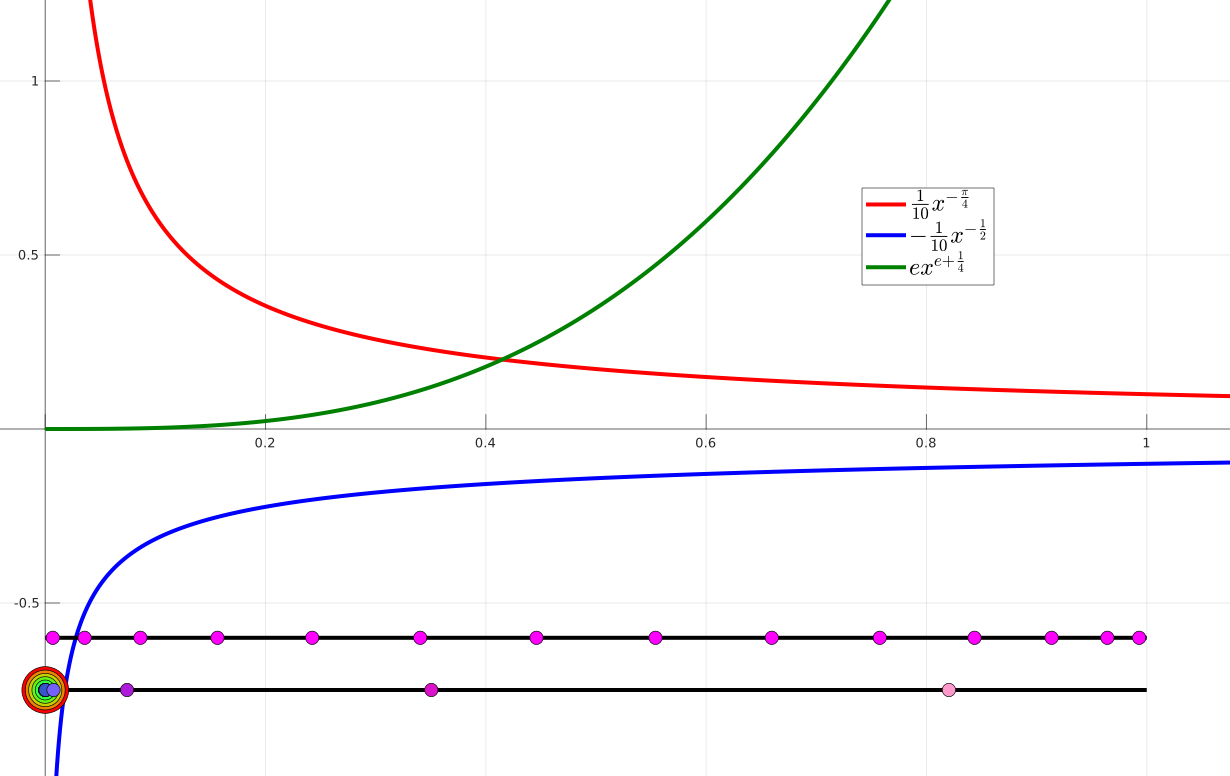
\includegraphics[keepaspectratio,width=\textwidth]{images/GenPolyMonMap.png}
        \caption{Plot of three generalised monomial terms of the Müntz polynomial $p(x)$ in (\ref{eq1.20}). On the bottom of the graph there is the distribution in $(0,1)$ of the $n=14$ nodes of a classical G-L formula (magenta) and the new samples obtained by the monomial transformation quadrature rule (linear color gradient). Due to the extreme clustering of the latter (see \ref{table1.2}), they are plotted with scaled-down circles as we move from $a=0$ to $b=1$. We clearly observe how classical G-L nodes in $(0,1)$ are insufficient to model the singular behaviour near $x=0$, causing a consistent loss in accuracy. On the other hand, the action of map $(\ref{eq1.16})$ on the nodes (whose order $r=28.77$ is given by (\ref{eq1.17})) re-arranges the vast majority of them around the endpoint singularities of $x^{-\frac{\pi}{4}}$ and $x^{-\frac{1}{2}}$, i.e. $x=0$.}
        \label{Fig1.2}
        \end{figure}
\end{center}

\newpage

\begin{table}[H]
\centering
\begin{tabular}{|c||c|c|c|c|}
\hline
& \multicolumn{2}{|c|}{\textbf{Classical G-L parameters}}&\multicolumn{2}{|c|}{\textbf{Monomial quadrature (QUASIMONT)}}\\
\hline
$j\in\mathbb{N}$ & $\tilde{x}_j\in(0,1)$ & $\tilde{w}_j\in\mathbb{R}^+$ & $x_j\in(0,1)$ & $w_j\in\mathbb{R}^+$ \\
\hline
1   &  0.00685809565159384 &  0.0175597301658759   &  5.58247922741512e-63  & 4.11231619931278e-61  \\
2   &  0.0357825581682132  &  0.0400790435798801   &  2.44695140063495e-42  & 7.88526679349951e-41  \\
3   &  0.0863993424651175  &  0.0607592853439516   &  2.52951532315787e-31  & 5.11781542764354e-30  \\
4   &  0.156353547594157   &  0.0786015835790968   &  6.51929796325047e-24  & 9.42908328714637e-23  \\
5   &  0.242375681820923   &  0.0927691987389689   &  1.95675667095192e-18  & 2.15474891008643e-17  \\
6   &  0.340443815536055   &  0.102599231860648    &  3.44180025480158e-14  & 2.98421017862521e-13  \\
7   &  0.445972525646328   &  0.107631926731579    &  8.13715952769522e-11  & 5.65003223119147e-10  \\
8   &  0.554027474353672   &  0.107631926731579    &  4.18125660540031e-08  & 2.33701617760019e-07  \\
9   &  0.659556184463945   &  0.102599231860648    &  6.30683776156361e-06  & 2.82259817558914e-05  \\
10   &  0.757624318179077   &  0.0927691987389689   &  0.000340288421120315  & 0.00119878736245905  \\
11  &  0.843646452405843   &  0.0786015835790968   &  0.00750950989496675   & 0.0201292451904070  \\
12  &  0.913600657534883   &  0.0607592853439516   &  0.0742930434150393    & 0.142150858859985  \\
13  &  0.964217441831787   &  0.0400790435798801   &  0.350516762468882     & 0.419175839329777  \\
14  &  0.993141904348406   &  0.0175597301658759   &  0.820378484398468     & 0.417316809008697  \\
\hline
\end{tabular}
  \caption{List of all the $n=14$ G-L nodes and weights before (classical) and after the application of the monomial transformation of order $r=28.77$ as depicted by Figure \ref{Fig1.2}.}
  \label{table1.2}
\end{table}

\chapter[Installation]{\Huge \ttfamily INSTALLATION}\chaptermark{INSTALLATION}

In the following chapter we illustrate how to build executable applications with QUASIMONT from its source code as well as the dependencies needed at link-time. We begin from the latter by outlining the third-party source code necessary for the library prior to the compilation itself. Later, a brief description of the organisation and structure of the code is given in order to facilitate the comprehension of the user interface at compile and link time. Then, we address how the library is actually built and illustrate its core features through the execution of some proposed test drivers. We remark that all of the following content regards the execution of QUASIMONT as a stand-alone software as we postpone to the next chapter the instructions needed to use our tool as a static library that is fully-integrable into a user's own application. Finally we address what has been originally mentioned in the opening lines of the first chapter of the present manual, that is that our package features two {\itshape modes} of execution, namely the \color{poliDarkBlue} \textbf{loud} \color{black} and \color{poliDarkBlue} \textbf{silent mode} \color{black}. Although the content of the present chapter is independent of the {\itshape mode} with which QUASIMONT is executed, we hereby refer exclusively to the former loud mode while for the latter we direct the user to Section \ref{Sec3.2} in which we address the main differences in I/O between the two.

\section[Third-party code]{\changefont THIRD-PARTY CODE}\sectionmark{THIRD-PARTY CODE}\label{Sec2.1}

\noindent
As reported in the opening section, QUASIMONT is entirely written in C++17; beside the speed and versatility of the language, the primary motivation behind such choice was the accessibility to other open-source packages. The library that we propose is composed by two modules with  corresponding \colorbox{poliGrayBlue}{main} functions. The {\itshape primary} module is the one used  to build executables and it implements all the essential methods that are required for the accomplishment of QUASIMONT's purpose, that is the computation of a monomial transformation quadrature rule that achieves double precision approximations of a definite integral whose integrands are generalized polynomials.  The {\itshape secondary} module provides supporting tools for the user's in-depth understanding of the fundamental blocks of the monomial transformation. It provides the plot of the asymptotic estimate $(\ref{eq1.8})$ and the computation of $\beta_{\text{min}}(n)$ and $\beta_{\text{min}}(n)$. As the secondary module is not essential for the correct functioning of the library (primary module), we kept it separated from the rest of the code, mainly because it introduces additional dependencies. In the following we address the main points concerning the primary module and we post-pone to Section \ref{Sec3.5} a brief description of the secondary module. QUASIMONT relies on a number of third-party open-source libraries. Many of them usually come shipped with C++ itself e.g. the \color{poliDarkBlue} \textbf{standard} \color{black} and \color{poliDarkBlue} \textbf{vector} \color{black} libraries (required for basic data-structures and functions), the \color{poliDarkBlue} \textbf{algorithm} \color{black} library (needed for sorting methods), the \color{poliDarkBlue} \textbf{math} \color{black} library (used for basic mathematical operations s.a. \colorbox{poliGrayBlue}{fabs}, \colorbox{poliGrayBlue}{pow} and \colorbox{poliGrayBlue}{ceil}) and others. The software also requires two more libraries that are well-known in the scientific computing and open-source communities; those are listed below with their minimum versions required for the correct build and execution of QUASIMONT reported between brackets:

\begin{itemize}
    \item \color{poliDarkBlue} \textbf{Boost C++ libraries (v-1.66)} \color{black}\cite{boost}: a vast, peer-reviewed, collection of mostly header source files. In particular QUASIMONT extensively uses the \colorbox{poliGrayBlue}{Multiprecision} library, where non-native higher precision f.p. formats have been implemented as C++ data-types. Of particular interest for our module is the IEEE 754 quadruple f.p. format which is supplied by Boost's library as GCC's \colorbox{poliGrayBlue}{\_\_float128} or Intel's \colorbox{poliGrayBlue}{\_Quad} types.
    \item \color{poliDarkBlue} \textbf{GSL - GNU Scientific Library (v-2.5)} \color{black}\cite{gsl}: required by QUASIMONT in only one instance, that is the computation of the roots of $(\ref{eq1.18})$ via the method \colorbox{poliGrayBlue}{gsl\_poly\_complex\_solve}. Alternative solvers and root-finders are available however in our case we were also interested in automatically locating the sole real root of such polynomial (corresponding to $n_{\text{min}}$ in $(\ref{eq1.18})$), hence the choice we made.
\end{itemize}

\noindent
These dependencies need to be installed/compiled correctly on the user's machine; furthermore macros to each static library need to be included in the standard search paths in order to correctly link the objects files compiled from the source code. All of the listed requirements are easily installed in Linux using package managers, such as the \color{poliDarkBlue} \textbf{Advanced Package Tool} \color{black} and the \color{poliDarkBlue} \textbf{Yellowdog Updater, Modified} \color{black} (or its successor \color{poliDarkBlue} \textbf{Dandified YUM}\color{black}), with a few commands on the terminal.

\vspace{0.2cm}
\begin{tcblisting}{enhanced,
                   arc=5mm,
                   title = \color{black}{\large \ttfamily Installation of third-party libraries},
                   colbacktitle=bashGray,
                   colback=bashBlue,
                   listing only,
                   listing style=BashStyle}
user@machine: home> # For Debian-based distros (Ubuntu, Mint, Knoppix, Kali ...)
user@machine: home> sudo apt-get update
user@machine: home> sudo apt-get install libboost-all-dev libgsl-dev
user@machine: home> # For RPM-based distros (CentOS, Fedora, SUSE, Scientific Linux ...)
user@machine: home> sudo dnf makecache --refresh
user@machine: home> sudo dnf install http://repo.okay.com.mx/centos/8/x86_64/release/okay-release-1-1.noarch.rpm
user@machine: home> sudo dnf install boost gsl libquadmath
user@machine: home> sudo dnf install boost-devel gsl-devel
\end{tcblisting}
\vspace{0.3cm}

\noindent
Additionally, QUASIMONT requires the proper installation of the appropriate building tools; at the present moment the library has been written for Linux platforms only and therefore we prioritized a minimalist and straightforward building process over cross-platform compliance by adopting the usage of {\itshape makefiles} (see Section \ref{Sec2.3}). The default compiler we selected for building QUASIMONT is the \color{poliDarkBlue} \textbf{GCC - GNU Compiler Collection} \color{black} \cite{gcc} that is invoked from the \color{poliDarkBlue} \textbf{GNU Make} \color{black} \cite{make} program. For this reason the installation of \colorbox{poliGrayBlue}{gcc} and \colorbox{poliGrayBlue}{make} are required on the user machine. Also in this case the aforementioned package managers allow fast and simple installation of the tools with minimal input on the terminal.

\vspace{0.2cm}
\begin{tcblisting}{enhanced,
                   arc=5mm,
                   title = \color{black}{\large \ttfamily Installation of building tools},
                   colbacktitle=bashGray,
                   colback=bashBlue,
                   listing only,
                   listing style=BashStyle}
user@machine: home> # For Debian-based distros (Ubuntu, Mint, Knoppix, Kali ...)
user@machine: home> sudo apt-get install build-essential
user@machine: home> gcc --version
user@machine: home> make --version
user@machine: home> # For RPM-based distros (CentOS, Fedora, SUSE, Scientific Linux ...)
user@machine: home> sudo dnf install gcc gcc-c++ make
user@machine: home> gcc --version
user@machine: home> make --version
\end{tcblisting}
\vspace{0.3cm}

\noindent
We remark that our QUASIMONT's built has been achieved using the minimum versions \colorbox{poliGrayBlue}{8.5.0} and \colorbox{poliGrayBlue}{4.2.1} of \colorbox{poliGrayBlue}{gcc} and \colorbox{poliGrayBlue}{make} respectively. We then tested its compilation and execution on three different platforms, namely using two Intel(R) Core(TM) i5-1035G1 @ 1.00GHz and i9-9900K @ 3.60GHz processors on a DEB-based \colorbox{poliGrayBlue}{Ubuntu 20.04.3} operating system (OS) and also a Intel(R) Core(TM) i7-10700 @ 2.90GHz processor on a RPM-based \colorbox{poliGrayBlue}{CentOS 8.5} OS (the last two running on virtual machines on a Windows host). Although the library has been tested in multiple development configurations that are compatible with the above listed requirements, the user may refer to Table \ref{table2.1} where we recap the information regarding the aforementioned authors' specific development environments. Once all the above packages have been installed, the user should thoroughly check the correct configuration, having care to particularly assure that links to the static libraries of each of the dependencies listed above have been added to \colorbox{poliGrayBlue}{gcc}'s linker \colorbox{poliGrayBlue}{ld} standard search paths.

\begin{table}[H]
\centering
\begin{tabular}{|c||c|c|c|c|c|c|c|c|}
\hline
\multicolumn{9}{|c|}{\textbf{Environments recap}} \\
\hline
Env. n. & OS (Unix) & Processor & GCC & Make & Boost & GSL & MPFR & GMP \\
\hline
1 & Ubuntu 20.04.3 & i5-1035G1 & 9.3.0 & 4.2.1 & 1.77 & 2.5 & 4.1.0 & 6.2.1 \\
2 & CentOS 8.5     & i7-10700  & 8.5.0 & 4.2.1 & 1.66 & 2.5 & 4.1.6 & 5.1.0 \\
\hline
\end{tabular}
  \caption{QUASIMONT Development environments used by the authors. The two rightmost columns refer to the secondary module of the library and are not a dependency requirement (see Section \ref{Sec3.5}).}
  \label{table2.1}
\end{table}

\noindent
The dependencies are constituted of large libraries, although QUASIMONT uses a limited amount of the methods they provide. We therefore made sure that only the necessary parts of the libraries are included in the source code, striving to maintain a clean and light final product. For the sake of completeness we hereby list all the methods of the selected third-party libraries  that are used by QUASIMONT.  These methods can be located in the source code, specifically in the header file \colorbox{poliGrayBlue}{Quasimont.h}, reported in the snippet below.

\vspace{0.2cm}
\tcbinputlisting{enhanced,
                 arc=5mm,
                 title = \color{black}{\large \ttfamily Quasimont.h},
                 colbacktitle=poliOrange,
                 colback=poliGrayBlue,
                 listing only,
                 listing style=CppStyle,
                 listing file=snippets/Quasimont.h}

\newpage

\noindent
As for any other source file in the library, a comment block precedes the code; in it the first line specifies the location of the specific file in the library's relative directory's tree (see Figure \ref{Fig2.1}). We only report such comment box for the above snippet of \colorbox{poliGrayBlue}{Quasimont.h} and omit it for any following snippet for the sake of space and clarity.

\vspace{0.2cm}
\tcbinputlisting{enhanced,
                 arc=5mm,
                 title = \color{black}{\large \ttfamily Quasimont.cpp},
                 colbacktitle=poliOrange,
                 colback=poliGrayBlue,
                 listing only,
                 listing style=CppStyle,
                 listing file=snippets/Quasimont.cpp}

\newpage
\noindent
We note that all the headers (and thus the declarations of all their methods) constituting the library (see Section \ref{Sec2.2}) are included in \colorbox{poliGrayBlue}{Quasimont.h}. Further below in the above header we find the definitions of the important constants that are used throughout the library which precede the declaration of the access point of the primary module of the library, i.e. the method \colorbox{poliGrayBlue}{quasimont} in which all other methods of QUASIMONT interact. The user may notices that we overloaded the primary module \colorbox{poliGrayBlue}{quasimont} method by taking different inputs and returning different outputs depending on whether the loud or silent mode is executed. We observe that compile-time polymorphism in C++ is not allowed when only the return type of the function differs which results in identical signatures. The definition for both modes of the method is given in the homonym source file \colorbox{poliGrayBlue}{Quasimont.cpp} reported above.

\section[Structure]{\changefont STRUCTURE}\sectionmark{STRUCTURE}\label{Sec2.2}

\noindent
The source-code in the library does not use relative paths for finding the definitions of its methods in the headers; relative paths are instead used at compile and link time by the \colorbox{poliGrayBlue}{makefile} (see Section \ref{Sec2.3}). The user is nonetheless discouraged from moving files and/or changing those paths because they do appear occasionally in the source code for retrieving data from specific non-source files. All of QUASIMONT's methods interact through the access point of the primary module \colorbox{poliGrayBlue}{quasimont} that interfaces the user through the inputs defined in the \colorbox{poliGrayBlue}{main} function. Apart from it, all the remaining source code that constitutes the primary module of the proposed software is made of only $12$ methods whose definitions are collected in one of the following three source files and related headers:

\begin{itemize}
    \item \colorbox{poliGrayBlue}{MonMap.cpp} contains every method associated with the computation of the monomial transformation quadrature rule, ranging from the monomial map itself (i.e. $\beta_{\text{min/max}}$ and $r$) to the quadrature parameters (i.e. $\tilde{x}_j$, $\tilde{w}_j$, $J_{[a,b]}$, etc...). To provide an easier reference for code debugging and amendment, a naming scheme of these methods is adopted. Every function in this file is in fact named \color{poliDarkBlue} \textbf{compute}$\boldsymbol{<}$\textbf{NameOfFunction$\boldsymbol{>}$} \color{black} as it can be evinced from the corresponding header file containing such functions' declarations
    
    \vspace{0.2cm}
    \tcbinputlisting{enhanced,
                 arc=5mm,
                 grow to left by=8mm, 
                 title = \color{black}{\large \ttfamily MonMap.h},
                 colbacktitle=poliOrange,
                 colback=poliGrayBlue,
                 listing only,
                 listing style=CppStyle,
                 listing file=snippets/MonMap.h}
    
    \newpage
    \item \colorbox{poliGrayBlue}{DatIo.cpp} is the source file defining each method that does not perform raw computations but instead manages the data flow e.g. in I/O operations. Every function follows the naming scheme \color{poliDarkBlue} $\boldsymbol{<}$\textbf{NameOfFunction$\boldsymbol{>}$}\textbf{Data} \color{black} emphasizing its characteristics of data manipulation method. The methods are declared in the header below
    
    \vspace{0.2cm}
    \tcbinputlisting{enhanced,
                 arc=5mm,
                 grow to left by=8mm,
                 title = \color{black}{\large \ttfamily DatIo.h},
                 colbacktitle=poliOrange,
                 colback=poliGrayBlue,
                 listing only,
                 listing style=CppStyle,
                 listing file=snippets/DatIo.h}
    \vspace{0.3cm}
    
    \item \colorbox{poliGrayBlue}{VecOps.cpp} defines every function that neither performs quadrature-related computations nor I/O data operations. Given their generic nature, no naming scheme is assigned to them as they are declared in \colorbox{poliGrayBlue}{Utils.h} alongside the $3$ methods of the secondary module defined in \colorbox{poliGrayBlue}{ErrTools.cpp} (see Section \ref{Sec3.5}).
    
    \vspace{0.15cm}
    \tcbinputlisting{enhanced,
                 arc=5mm,
                 grow to left by=8mm,
                 grow to right by=2mm,
                 title = \color{black}{\large \ttfamily Utils.h},
                 colbacktitle=poliOrange,
                 colback=poliGrayBlue,
                 listing only,
                 listing style=CppStyle,
                 listing file=snippets/Utils.h}
\end{itemize}

\noindent
With reference to Figure \ref{Fig2.1} we present a visual sketch of the files' organisation in the library's directory. Source files of the primary module, i.e. \colorbox{poliGrayBlue}{MonMap.cpp} and \colorbox{poliGrayBlue}{DatIo.cpp} are located in the subdirectory \colorbox{poliGrayBlue}{\textbf{QUASIMONT/src}} alongside \colorbox{poliGrayBlue}{Quasimont.cpp}. On the other hand the \colorbox{poliGrayBlue}{VecOps.cpp} source file is instead placed in the supplementary \colorbox{poliGrayBlue}{\textbf{QUASIMONT/utilities}} subdirectory where we can also find the secondary module's source code \colorbox{poliGrayBlue}{ErrTools.cpp}. Despite such separation, all the header files outlined above are located in the \colorbox{poliGrayBlue}{\textbf{QUASIMONT/include}} subdirectory, including \colorbox{poliGrayBlue}{Quasimont.h}. We recall that some relative paths are essential for the correct loading of raw data from \color{poliDarkBlue} \textbf{tabulated data-files} \color{black} into the source code.

\begin{center}
        \begin{figure}[H]
        \centering
        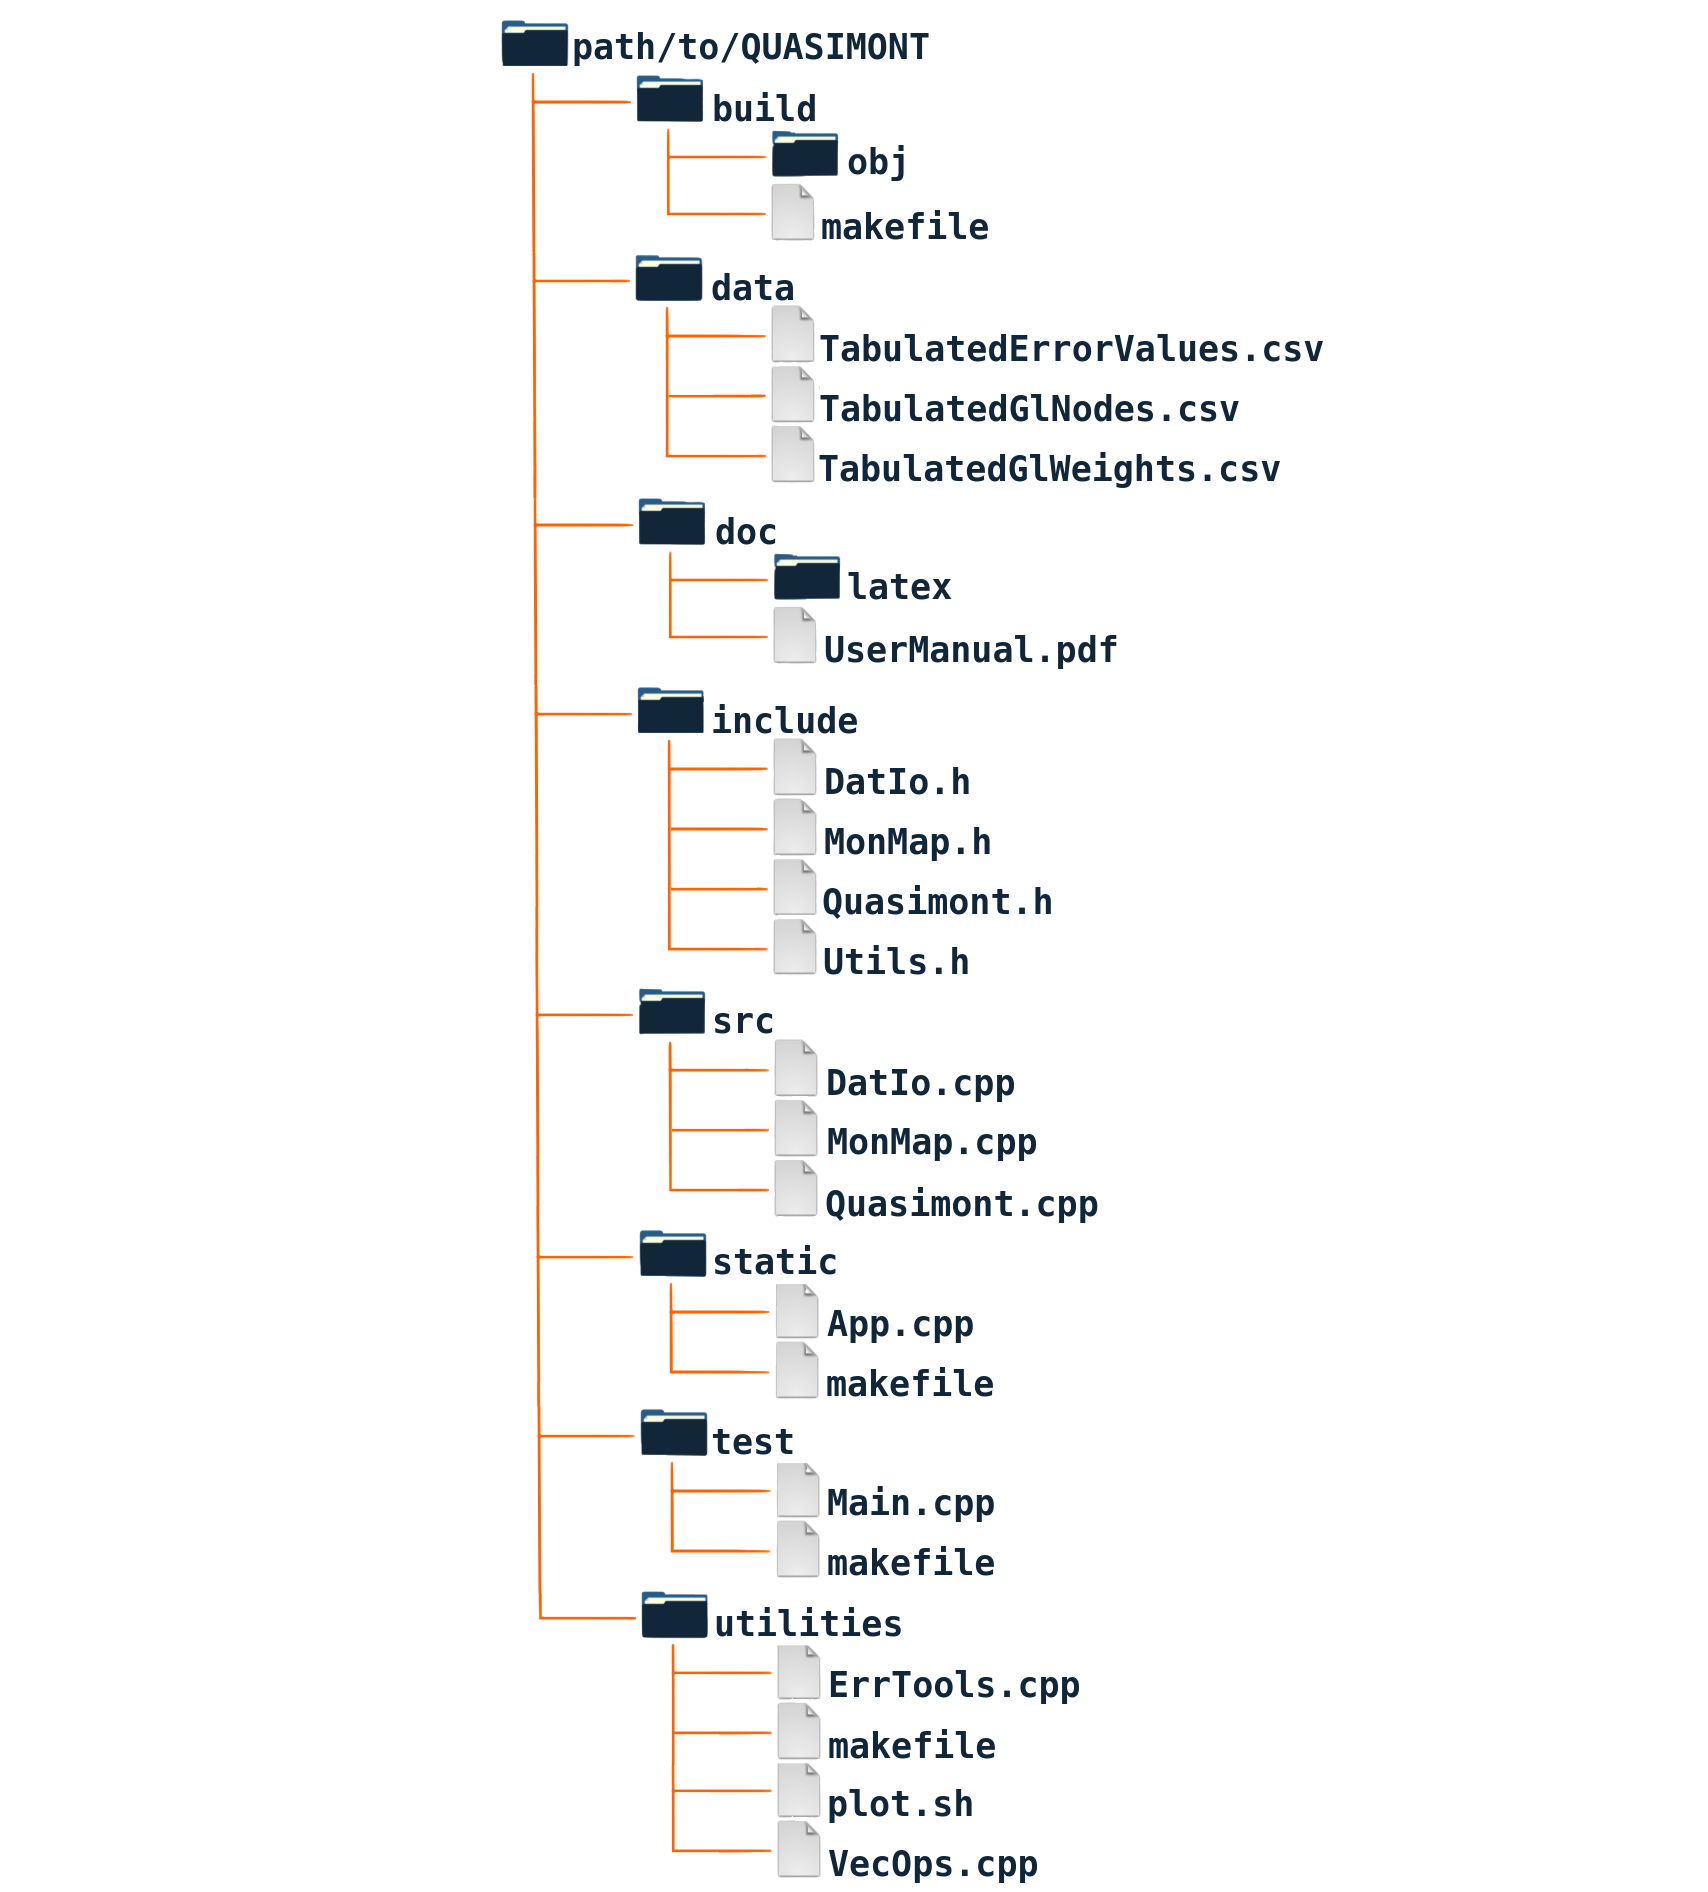
\includegraphics[keepaspectratio, width=.6\textwidth]{images/DirectoryStructureCentered.png}
        \caption{The directory tree representing the structure and organisation of QUASIMONT}
        \label{Fig2.1}
        \end{figure}
\end{center}

\noindent 
 Those files are:
\begin{itemize}
    \item \colorbox{poliGrayBlue}{TabulatedErrorValues.csv} collecting the values of $\beta_{\text{min}}(n)$ and $\beta_{\text{max}}(n)$ for each even value of $n\in[10,100]$;
    \item \colorbox{poliGrayBlue}{TabulatedGlNodes.csv} storing the G-L quadrature nodes in $[-1,1]$ for each even value of $n\in[10,100]$;
    \item \colorbox{poliGrayBlue}{TabulatedGlWeights.csv} storing the weights of the G-L quadrature formula for each even value of $n\in[10,100]$.
\end{itemize}
We note that the latter two tabulated values of the original G-L nodes and weights in $(-1,1)$ are stored with $50$ decimal digits of precision. Their automatic computation is outside the scope of the library and already explored in details and implemented in other works \cite{Gautschi94,Hale13}. Those files are located in \colorbox{poliGrayBlue}{\textbf{QUASIMONT/data}} and shall never be edited. In the \colorbox{poliGrayBlue}{\textbf{QUASIMONT/build}} the \colorbox{poliGrayBlue}{makefile} used for building the library and its applications is located whereas \colorbox{poliGrayBlue}{\textbf{QUASIMONT/build/obj}} subdirectory contains the object files created at compile-time. Finally, test drivers (see Section \ref{Sec2.4}) used for checking the proper installation and execution of the application are located in \colorbox{poliGrayBlue}{\textbf{QUASIMONT/test}} while in \colorbox{poliGrayBlue}{\textbf{QUASIMONT/static}} we stored an example application for compiling and using the static library version of our software (see Section \ref{Sec3.3}).

\newpage
\section[Build process]{\changefont BUILD PROCESS}\sectionmark{BUILD PROCESS}\label{Sec2.3}

\noindent
QUASIMONT is a quadrature tool that can be easily integrated in  users' applications, while creating executables. In the provided library, the integration is performed, for example, through the compilation and linking of the library's source code with a \colorbox{poliGrayBlue}{Main.cpp} file containing the user's input, thus called \color{poliDarkBlue} \textbf{input source file} \color{black} (see Section \ref{Sec3.1}). This file determines the {\itshape gateway} for the access point \colorbox{poliGrayBlue}{quasimont} of the primary module and therefore there should be one in any application built by the user. This is due to a fundamental rule in C++, for which only one \colorbox{poliGrayBlue}{main} is defined at global level. By design, in our library, \colorbox{poliGrayBlue}{quasimont} method acts as the designated {\itshape entry point} of the monomial transformation quadrature algorithm at run-time.

\vspace{0.2cm}
\tcbinputlisting{enhanced,
                 arc=5mm,
                 title = \color{black}{\large \ttfamily Application's own (top-level) makefile},
                 colbacktitle=poliOrange,
                 colback=poliGrayBlue,
                 listing only,
                 listing style=MakeStyle,
                 listing file=snippets/makefile}
\vspace{0.3cm}

\noindent
The source code of the library itself (i.e. the source files in \colorbox{poliGrayBlue}{\textbf{QUASIMONT/src}}) does not define any \colorbox{poliGrayBlue}{main} function and thus can only be compiled but not executed by itself. In order to build applications, the compiled source code has to be linked with a compiled \colorbox{poliGrayBlue}{main} that provides the access point of the primary module to the program's executable. We can define a sort of one-to-one correspondance between each application's executable and its associated \colorbox{poliGrayBlue}{main} function, the latter uniquely identified by the input singular generalised polynomials defined by the user. The build process is based on a \textsl{recursive make} approach, i.e. the input source file is built through a top-level \colorbox{poliGrayBlue}{makefile} (reported above) that recursively invokes the \colorbox{poliGrayBlue}{makefile} responsible for building the source code of the library, its utilities and third-party dependencies. The library source code shall be compiled just once and the resulting objects shall remain available thereafter for linking to any \colorbox{poliGrayBlue}{main}, i.e. new applications. Whenever the rule \colorbox{poliGrayBlue}{allclean} is invoked from the top-level \colorbox{poliGrayBlue}{makefile}, it deletes those object files and the source code does require to be compiled again. This practice is useful for users who require to execute standalone applications by reusing the unchanged compiled objects of the source code multiple times. In these cases we remark that the output consists of the specialised quadrature samples in addiction to the numerical estimation of the integral for a generalised polynomial. Such output data is stored in a specific sub-directory as described in Section \ref{Sec3.2}.

\vspace{0.2cm}
\begin{tcblisting}{enhanced,
                   arc=5mm,
                   title = \color{black}{\large \ttfamily Compilation and Linking of the library},
                   colbacktitle=bashGray,
                   colback=bashBlue,
                   listing only,
                   listing style=BashStyle}
# First clean the object files from any previous compilation
user@machine: home/QUASIMONT/test> make allclean
make clean
make[1]: Entering directory '/home/QUASIMONT/test'
rm -f ../build/obj/Main.o Test
if [ -d "output" ]; then rm -r output; fi 
make[1]: Leaving directory '/home/QUASIMONT/test'
cd ../utilities && make clean
make[1]: Entering directory '/home/QUASIMONT/utilities'
rm -f Tools && if [ -d "estimate" ]; then rm -r estimate; fi
rm -f ../build/obj/*.o
make[1]: Leaving directory '/home/QUASIMONT/utilities'
cd ../build && make clean
make[1]: Entering directory '/home/QUASIMONT/build'
rm -f obj/*.o
make[1]: Leaving directory '/home/QUASIMONT/build'
# Then the build starts by compiling the library source into object files
user@machine: home/QUASIMONT/test> make
g++ -c Main.cpp -o ../build/obj/Main.o -ansi -std=c++17 -I ../include
cd ../build && make
make[1]: Entering directory '/home/QUASIMONT/build'
g++ -c ../src/Quasimont.cpp -o obj/Quasimont.o -g -ansi -std=c++17 -I ../include 
g++ -c ../src/DatIo.cpp -o obj/DatIo.o -g -ansi -std=c++17 -I ../include 
g++ -c ../src/MonMap.cpp -o obj/MonMap.o -g -ansi -std=c++17 -I ../include 
make[1]: Leaving directory '/home/QUASIMONT/build'
cd ../utilities && make ../build/obj/VecOps.o
make[1]: Entering directory '/home/QUASIMONT/utilities'
g++ -c VecOps.cpp -o ../build/obj/VecOps.o -g -ansi -std=c++17 -I ../include 
make[1]: Leaving directory '/home/QUASIMONT/utilities'
# Once all the objects have been compiled the linker automatically generates the executable and launches the simulation
g++ ../build/obj/*.o -o Test -lm -lquadmath -lgsl -lgslcblas
./Test

    |-------------------------------------------------|
    |                 ** QUASIMONT **                 |
    |  ** MONOMIAL TRANSFORMATION QUADRATURE RULE **  |
    |-------------------------------------------------|


 Input polynomial p(x) = ...
\end{tcblisting}
\vspace{0.3cm}

\noindent
On the other hand, if integration of QUASIMONT in larger more complex software is required (e.g. in FEM/BEM libraries), linking to the static library is necessary, which is addressed later in the manual at Section \ref{Sec3.3}. Regardless, during compilation it may happen that, depending on the distro and version of \colorbox{poliGrayBlue}{gcc} used, the user is prompted with the following \colorbox{poliGrayBlue}{error: unable to find numeric literal operator 'operator''''Q'}. In such case the user must append the \colorbox{poliGrayBlue}{-fext-numeric-literals} flag to the \colorbox{poliGrayBlue}{CXXOPTIONS} macro as reported in the above \colorbox{poliGrayBlue}{makefile} snippet and all the remaining ones in the library (see Section \ref{Sec2.2} and Figure \ref{Fig2.1}). To conclude the discussion on how the QUASIMONT is built locally, let us display the outcome of some of the basic rules defined in the top-level \colorbox{poliGrayBlue}{makefile}. The output of the compilation of the source files are object files that are stored in the \colorbox{poliGrayBlue}{\textbf{QUASIMONT/build/obj}} subdirectory. The linking of those objects is invoked only by the top-level makefile associated to the specific application. For each application built by the user it is considered a good practice to invoke the \colorbox{poliGrayBlue}{clean} rule prior to the build process itself. We emphasize that, with the exception of those cases when QUASIMONT is used as a tool in a larger library, each application should be associated to its own subdirectory located within QUASIMONT itself. In this subdirectory a user input source file containing the \colorbox{poliGrayBlue}{main}, named \colorbox{poliGrayBlue}{Main.cpp} by default, should be located. User may opt for changing the filename of \colorbox{poliGrayBlue}{main} as it does not impact any aspect of the source code as long as the same name appears in the \colorbox{poliGrayBlue}{default} rule reported in the top-level \colorbox{poliGrayBlue}{makefile} of the application, which should also be located in the subdirectory. For simplicity, we suggest to retain the naming convention reported in the provided \colorbox{poliGrayBlue}{makefile}. In this scheme, the application's name (in our example \colorbox{poliGrayBlue}{Test}) matches that of the directory in which its input source file \colorbox{poliGrayBlue}{Main.cpp} is located (i.e. \colorbox{poliGrayBlue}{\textbf{QUASIMONT/test}}). In the next subsection a reference application located in  \colorbox{poliGrayBlue}{\textbf{QUASIMONT/test}} (already shipped with the library) exemplifies the whole build sequence.

\section[Installation and test driver]{\changefont INSTALLATION AND TEST DRIVER}\sectionmark{INSTALLATION AND TEST DRIVER}\label{Sec2.4}

\noindent
The installation of the library can be done by building the \colorbox{poliGrayBlue}{Main.cpp} input source file in the \colorbox{poliGrayBlue}{\textbf{QUASIMONT/test}} subdirectory, which contains the test driver for benchmarking QUASIMONT's performance. The \colorbox{poliGrayBlue}{Test} application  runs the library's processing methods for three generalised and classical polynomial, thus introducing the user to its execution and interaction whilst assuring that the core functionalities have been compiled correctly (no conflict at linking stage occurs). The three polynomial functions are the following

\begin{equation*}
    \begin{split}
        p_1(x) & = 5x^{-\frac{\pi}{4}}-x^{-\frac{1}{2}}+1+10x^{2}+ex^{e+\frac{1}{4}} \\
        p_2(x) & = x^{-\frac{e}{3}} \\
        p_3(x) & = x^{17} + x^{35}
    \end{split}
\end{equation*}

\noindent
and, with the exception of $p_3(x)$, all have a singularity in $x=0$ (QUASIMONT defaults the integration interval to be $(0,1)$). Once the library's and the input source file have been compiled and linked into the corresponding executable, the resulting application integrates each polynomial using the monomial transformation quadrature rule. We remark that, although no difference in numerical results occurs, the following report solely concerns the loud mode of execution. A list of information regarding the monomial transformation itself is displayed on the terminal whereas the results of interest (i.e. the new processed quadrature together with the related numerical integration) \color{black} are exported in files located in the appropriate output directory (see Section \ref{Sec3.2}). 

\vspace{0.2cm}
\begin{tcblisting}{enhanced,
                   arc=5mm,
                   title = \color{black}{\large \ttfamily Building and executing the test driver: p\_1(x)},
                   colbacktitle=bashGray,
                   colback=bashBlue,
                   listing only,
                   listing style=BashStyle}
user@machine: home/QUASIMONT/test> make clean
make clean
rm -f ../build/obj/Main.o Test
if [ -d "output" ]; then rm -r output; fi
user@machine: home/QUASIMONT/test> make
g++ -c Main.cpp -o ../build/obj/Main.o -ansi -std=c++17 -I ../include
g++ ../build/obj/*.o -o Test -lm -lquadmath -lgsl -lgslcblas
./Test

    |-------------------------------------------------|
    |                 ** QUASIMONT **                 |
    |  ** MONOMIAL TRANSFORMATION QUADRATURE RULE **  |
    |-------------------------------------------------|

 Input polynomial p(x) =  +2.71828183*x^(2.96828183) +5*x^(-0.785398163) -1*x^(-0.5) +x^(0)  +10*x^(2)

 ** Accepted sequence of exponents ** 
    {2.96828183, -0.785398163, -0.5, 0, 2}
 ** Lambda_min = -0.785398163, Lambda_max = 2.96828183 **
 --------------------------------------------------
 ** N_min = 32
 ** Beta_min = 4.37782519, Beta_max = 127.894326 **
 ** Transformation order = 28.7703455 **
 --------------------------------------------------
 ** Using double f.p. format for nodes and weights **
 ** I(p(x))   = 26.317297376488324 **
 ** I_n(p(x)) = 26.317297376488324      [with parameters in float128 precision] **
 ** E_n(p(x)) = 1.3889468142066847e-17  [with parameters in float128 precision] **
 ** I_n(p(x)) = 26.317297376488324      [with parameters in double precision] **
 ** E_n(p(x)) = 5.4523153678583704e-18  [with parameters in double precision] **

 ** QUASIMONT HAS TERMINATED **
\end{tcblisting}

\noindent
To check the correctness of the built application, the user should verify that the results obtained do indeed match the output data reported in the following tables \ref{table2.2}, \ref{table2.3}, \ref{table2.4} for each polynomial function. To run each benchmark the user needs to return to the CLI where the program is waiting for her/him to go ahead to the next case. Note that, since we are implementing three benchmark polynomials in a single source file, such pause is necessary during the execution in order to capture the new processed quadrature together with the associated numerical integration as the files in the output directory are overwritten at each execution. The correct execution of all three benchmarks will then close the application. The user should check that each benchmark is executed without problems and the results are correctly generated (see Section \ref{Sec3.2}). As for the quality of the results obtained for those tests, an in-depth analysis, coupled with the fast execution of the program, shows the advantages provided by QUASIMONT over classical G-L and other generalised quadrature rules. The first polynomial $p_1(x)$ is a model proposed in equation (73) of \cite{Lombardi09}, \textsl{Section 5.1, Example 1}, and it represents the typical integrand function often encountered in numerical methods for differential and integral equations featuring singular modelling, on which QUASIMONT is indeed considered an helpful, effective and precise tool. The proposed generalised polynomial $p_1(x)$ features a strong singularity at $x=0$ in the interval $(0,1)$ and all but two of its monomial terms have non-integer degree. The numerical approximation of the integral at double precision is achieved with $n=32$ nodes using a monomial transformation applied to the classical G-L quadrature with $n$ nodes in $(0,1)$. The Table \ref{table2.2} below shows what was graphically reported in Figure \ref{Fig1.2} i.e. the ad-hoc suited and more efficient distribution of the samples obtained by the monomial transformation as opposed to the ones of the classical G-L quadrature rule.

\vspace{0.2cm}
\begin{table}[H]
\centering
\begin{tabular}{|c||c|c|}
\hline
\multicolumn{3}{|c|}{\textbf{Nodes and weights of the proposed quadrature for $p_1(x)$ }} \\
\hline
$j\in\mathbb{N}$ & $x_j\in(0,1)$ & $w_j\in\mathbb{R}^+$ \\
\hline
1   &  4.0256721894941735e-83  &  2.9709584266857193e-81  \\
2   &  2.2116841854653406e-62  &  7.1971053989801097e-61  \\
3   &  3.4370358897566318e-51  &  7.1255611223692978e-50  \\
4   &  1.6010758830624544e-43  &  2.4253789034229506e-42  \\
5   &  1.0479208102676717e-37  &  1.2456363438765983e-36  \\
6   &  4.8718071131884711e-33  &  4.7453741025535338e-32  \\
7   &  3.7119919463646725e-29  &  3.0494845207591382e-28  \\
8   &  7.5510919371932376e-26  &  5.3393428605147779e-25  \\
9   &  5.58947068987428e-23    &  3.4526789629984772e-22  \\
10  &  1.8549840400142102e-20  &  1.0121884313459638e-19  \\
11  &  3.1981531227726135e-18  &  1.5545919457374846e-17  \\
12  &  3.1905126409913618e-16  &  1.3904418738462426e-15  \\
13  &  1.9974633805093215e-14  &  7.8421013950383668e-14  \\
14  &  8.3548669580378659e-13  &  2.9653252968844048e-12  \\
15  &  2.4525558094710645e-11  &  7.8879379262599627e-11  \\
16  &  5.2553535644885825e-10  &  1.5337625816699302e-09  \\
17  &  8.4865615532959245e-09  &  2.2485149221054993e-08  \\
18  &  1.0601166175497224e-07  &  2.5487504629916981e-07  \\
19  &  1.0467771915132323e-06  &  2.2805293469267595e-06  \\
20  &  8.3187859060800558e-06  &  1.6383778757563812e-05  \\
21  &  5.4017656350748472e-05  &  9.583886949817516e-05   \\
22  &  0.00029027719974030597  &  0.00046172220499588948  \\
23  &  0.0013048618829373392   &  0.0018488842315729846   \\
24  &  0.0049515587664587246   &  0.0061972140073356637   \\
25  &  0.01598386920155067     &  0.017474549464975012    \\
26  &  0.044176504650425052    &  0.041563995305652503    \\
27  &  0.10510275956828145     &  0.083385319613667491    \\
28  &  0.21621415218381346     &  0.14051580648196024     \\
29  &  0.38598199665949656     &  0.19670495174814193     \\
30  &  0.59964365548997856     &  0.22295968412650397     \\
31  &  0.81242716007987004     &  0.1915755472071223      \\
32  &  0.96137880664253184     &  0.097197543454586643    \\
\hline
\end{tabular}
  \caption{Nodes and weights obtained by a monomial transformation of order $r=28.77$ applied to the G-L quadrature integrating $p_1(x)$ in $(0,1)$ at double precision with $n=32$ samples.}
  \label{table2.2}
\end{table}

\noindent
While in fact we know that the $n=32$ nodes of the classical G-L quadrature rule are distributed symmetrically in $(0,1)$ with an equal abundance of those at both bounds of the integration interval, our proposed quadrature scheme, based on the monomial transformation, concentrates the samples close to the lower bound $x=0$, squashing the vast majority of them ($26$ out of the total $32$) inside the sub-interval $(0,0.1)$ thereby better capturing the singular behaviour of $p_1(x)$. The second benchmark polynomial is proposed with the scope of introducing the user to a core functionality of QUASIMONT that requires further input on the CLI. Indeed, $p_2(x)$ is a monomial of non-integer degree and its numerical integration requires careful manipulation. During the modelling process of larger applications, especially when dealing with finite elements constructed over meshed domains with singular spatial geometry behaviour \cite{Graglia04,Graglia08} it is often necessary to integrate low-order singular generalised polynomial basis functions together with high-order regular polynomial basis functions. QUASIMONT allows to integrate such integrals identifying the degree of the monomial as $\lambda_{\text{min}}$ and the maximum degree  $\lambda_{\text{max}}$ of the all set of combined polynomial functions. For this reason, in this test, we add a monomial with $\lambda_{\text{max}}$ degree and unitary coefficient to $p_2(x)$. Once constructed the final polynomial we apply the proposed algorithm to process the optimised nodes and weights. The integration is enabled using a caveat prompted on the terminal and it consists in choosing one path between two mutually exclusive options that the user must exercise in order to continue with the application.

\vspace{0.2cm}
\begin{tcblisting}{enhanced,
                   arc=5mm,
                   title = \color{black}{\large \ttfamily Building and executing the test driver: p\_2(x)},
                   colbacktitle=bashGray,
                   colback=bashBlue,
                   listing only,
                   listing style=BashStyle}
    |-------------------------------------------------|
    |                 ** QUASIMONT **                 |
    |  ** MONOMIAL TRANSFORMATION QUADRATURE RULE **  |
    |-------------------------------------------------|

 Input polynomial p(x) =  +x^(-0.906093943) 

 ** WARNING ** Your input is a monomial of non-integer degree.
               QUASIMONT needs a binomial for double-precision quadrature.
               How do you proceed? ['nodes' for n_min ~ 'lambda' for lambda_max]
               Input: 
\end{tcblisting}
\vspace{0.3cm}

\noindent
One of those is the choice of specifying the maximum number $n$ for the quadrature rule, in which case the library  automatically compute $\lambda_{\text{max}}$ and integrate $\tilde{p_2}(x) = x^{-\frac{e}{3}} + x^{\lambda_\text{max}}$ accordingly. The second path allows instead to specify $\lambda_{\text{max}}$ directly and let QUASIMONT carry out the integration. It is easy to see that the second case reduces to a \textsl{"standard"} polynomial input, as far as the library is concerned. The user should therefore type \colorbox{poliGrayBlue}{nodes} on the CLI and press Enter; we are now prompted to select any value of $n\in[10,100]$; user should type, for example, $64$ and press Enter again. On the contrary typing \colorbox{poliGrayBlue}{lambda} causes the application to resort to its original workflow with the additional intermediate step of requiring the input value of $\lambda_{\text{max}}$. We remark that any miss-typed or empty input results in QUASIMONT to throw an error message and exit the program. 

\vspace{0.2cm}
\begin{tcblisting}{enhanced,
                   arc=5mm,
                   title = \color{black}{\large \ttfamily Building and executing the test driver: p\_2(x)},
                   colbacktitle=bashGray,
                   colback=bashBlue,
                   listing only,
                   listing style=BashStyle}
Please specify the desired number of quadrature nodes (number must be even): 64
 --------------------------------------------------
 ** N_min = 64
 ** Beta_min = 3.25021668, Beta_max = 511.19448 **
 ** Accepted sequence of exponents ** 
    {-0.906093943, 10.3166381}
 ** Lambda_min = -0.906093943, Lambda_max = 10.3166381 **
 --------------------------------------------------
 ** N_min = 64
 ** Beta_min = 3.25021668, Beta_max = 511.19448 **
 ** Transformation order = 45.2603038 **
 --------------------------------------------------
 ** Using double f.p. format for nodes and weights **
 ** I(p(x))   = 10.737305800857456 **
 ** I_n(p(x)) = 10.737305800857441     [with parameters in float128 precision] **
 ** E_n(p(x)) = 1.424785764850455e-15  [with parameters in float128 precision] **
 ** I_n(p(x)) = 10.737305800857441     [with parameters in double precision] **
 ** E_n(p(x)) = 1.4344708669352776e-15 [with parameters in double precision] **

 ** QUASIMONT HAS TERMINATED **
\end{tcblisting}

\noindent
After the specified selection, QUASIMONT computes automatically a value of $\lambda_{\text{max}} = 10.3166381$ for $p_2(x)$ and the resulting quadrature barely retains the machine-epsilon double precision for the relative error of the numerical integration. Here, the library is stressed more as it can be evinced by the substantially greater value of the transformation order $(r=45.2603038)$ w.r.t. the previous instance in $p_1(x)$. The effects of such magnitude for the monomial transformation order are easily registered by assessing the mapped nodes and weights listed in the following table. Furthermore we highlight how the relative error obtained with \colorbox{poliGrayBlue}{float128} monomial transformation quadrature rule's parameters is not substantially better than the one derive with the same nodes and weights optimised in double f.p. format. In fact we observe that the latter format has been selected despite being slightly less precise than the former. The logic behind is that both relative errors are computed at run-time and if their absolute difference is smaller than twice the machine-epsilon in double precision than we go ahead and export the data in the most optimised format.

\begin{table}[H]
\hspace{-1.4cm}
\begin{tabular}{|c||c|c||c||c|c|}
\hline
\multicolumn{6}{|c|}{\textbf{Nodes and weights of the proposed quadrature for $p_2(x)$}} \\
\hline
$j\in\mathbb{N}$ & $x_j\in(0,1)$ & $w_j\in\mathbb{R}^+$ & $j\in\mathbb{N}$ & $x_j\in(0,1)$ & $w_j\in\mathbb{R}^+$ \\
\hline
1   & 2.7630147554775799e-157   & 3.2089404684705014e-155  & 33  & 7.0500634584281311e-14 & 1.5167370865604578e-13 \\
2   & 1.2504818169246583e-124   & 6.4130575288015817e-123  & 34  & 5.7559583188242479e-13 & 1.1793837946815465e-12 \\
3   & 5.6814585252048909e-107   & 1.8611939310882479e-105  & 35  & 4.2517694749483687e-12 & 8.2956748948158666e-12 \\
4   & 7.80153953804910668e-95   & 1.8746032945680622e-93   & 36  & 2.8538360103496875e-11 & 5.3006402608938980e-11 \\
5   & 1.37705792986285616e-85   & 2.6096113660080927e-84   & 37  & 1.7474698043212560e-10 & 3.0884893242340361e-10 \\
6   & 3.99955200879667989e-78   & 6.2503681667652076e-77   & 38  & 9.7966474232194539e-10 & 1.6467041924026613e-09 \\
7   & 7.12412148203568704e-72   & 9.4622687681839969e-71   & 39  & 5.0450425037572576e-09 & 8.0595541550951593e-09 \\
8   & 1.67758621116242340e-66   & 1.9352874634013771e-65   & 40  & 2.3937780380919019e-08 & 3.6314704984080236e-08 \\
9   & 8.50394804246417862e-62   & 8.6610446966327004e-61   & 41  & 1.0493924006829552e-07 & 1.5103117353143750e-07 \\
10  & 1.28937420430520282e-57   & 1.17417554134314e-56     & 42  & 4.2611947777521824e-07 & 5.8115902014625234e-07 \\
11  & 7.37695543314284930e-54   & 6.0678528535818764e-53   & 43  & 1.6064924620227659e-06 & 2.0734907170162103e-06 \\
12  & 1.88823854215581744e-50   & 1.4144870181471483e-49   & 44  & 5.6352337753679891e-06 & 6.8727595063813297e-06 \\
13  & 2.45874041791221323e-47   & 1.6888846224093984e-46   & 45  & 1.8428406102394049e-05 & 2.1200152242057246e-05 \\
14  & 1.79879095499131601e-44   & 1.1394463566176748e-43   & 46  & 5.6285102084355121e-05 & 6.0953635295967037e-05 \\
15  & 7.99644755427870559e-42   & 4.6939290576395100e-41   & 47  & 0.000160824501490444   & 0.00016357104996692    \\
16  & 2.30031834550869425e-39   & 1.256455692921632e-38    & 48  & 0.000430554366218858   & 0.000410178545783102   \\
17  & 4.50736224431423266e-37   & 2.2990244539015347e-36   & 49  & 0.001081507980701627   & 0.00096212522184789    \\
18  & 6.27605017641916653e-35   & 2.9984883056622040e-34   & 50  & 0.002552202028188329   & 0.002112665166000562   \\
19  & 6.43329661193267433e-33   & 2.8866958399889620e-32   & 51  & 0.005664918590851289   & 0.004345383033450631   \\
20  & 5.00167986643949820e-31   & 2.1127162036193374e-30   & 52  & 0.011839418057758923   & 0.008374932123081819   \\
21  & 3.02522544694279073e-29   & 1.2053618210763572e-28   & 53  & 0.023321020012667499   & 0.015126268661501289   \\
22  & 1.45485132139284000e-27   & 5.4774213217611214e-27   & 54  & 0.043333892814950261   & 0.025596514741963807   \\
23  & 5.66857779784746315e-26   & 2.0197293557945103e-25   & 55  & 0.076017823001042698   & 0.040555711474099192   \\
24  & 1.81901613177956244e-24   & 6.1417478949789698e-24   & 56  & 0.1259851142914331     & 0.060094184332119245   \\
25  & 4.87674410785629622e-23   & 1.5621281667244454e-22   & 57  & 0.197384568387222875   & 0.083114399815460055   \\
26  & 1.10619188116815056e-21   & 3.3648881412038240e-21   & 58  & 0.292508401834271963   & 0.106964653637029898   \\
27  & 2.14674169704207817e-20   & 6.2062442929374053e-20   & 59  & 0.410207778274644215   & 0.127463313674079491   \\
28  & 3.59979724510255679e-19   & 9.8975903331295861e-19   & 60  & 0.544613347654060773   & 0.139504287218888873   \\
29  & 5.26211017870698955e-18   & 1.3767307083491291e-17   & 61  & 0.68476273369408191    & 0.138243738177407818   \\
30  & 6.75862034692174972e-17   & 1.68331269687316e-16     & 62  & 0.815603424165963892   & 0.120596149243306058   \\
31  & 7.68166812405570700e-16   & 1.8218265936883635e-15   & 63  & 0.920443566774952144   & 0.086540144565319482   \\
32  & 7.77553771704852579e-15   & 1.756314510825820e-14    & 64  & 0.984393322175774548   & 0.039739900698273792   \\
\hline
\end{tabular}
  \caption{Nodes and weights obtained by a monomial transformation of order $r=45.26$ applied to the G-L quadrature integrating $p_2(x)$ in (0,1) at double precision with $n=64$ samples.}
  \label{table2.3}
\end{table}

\noindent
Finally, with the last benchmark a classical polynomial of high integer-degree is integrated; indeed, $p_3(x)$ is a binomial. For standard, polynomials we compare the performance of standard  G-L quadrature with the one of QUASIMONT. According to the properties described in Sub-Section \ref{SubSec1.2.2}, the former requires $n=\frac{\lambda_{max}+1}{2}=18$ nodes to achieve double precise integration however, we immediately realise that our library (more sepcifically the monomial transformation quadrature rule) outperforms the classical G-L quadrature rule for a fixed double precision accuracy as only $n=12$ samples are needed. We also remark  that the transformation order needed by the monomial map is significantly lower than the previous two cases, in particular less than $1$.

\newpage
\noindent
Since $p_3(x)$ does not have a singularity at $x=0$, the processing of G-L quadrature yields a monomial transformation quadrature with samples that are not clustered on $x=0$. In this instance instead, the transformation forces the performance of the quadrature to effectively integrate generalised polynomials with $\lambda\in\{17,35\}$ with machine-epsilon precision specified for the double f.p. format, as it can be assessed by the table below.

\vspace{0.2cm}
\begin{tcblisting}{enhanced,
                   arc=5mm,
                   title = \color{black}{\large \ttfamily Building and executing the test driver: p\_3(x)},
                   colbacktitle=bashGray,
                   colback=bashBlue,
                   listing only,
                   listing style=BashStyle}           
    |-------------------------------------------------|
    |                 ** QUASIMONT **                 |
    |  ** MONOMIAL TRANSFORMATION QUADRATURE RULE **  |
    |-------------------------------------------------|
    
Input polynomial p(x) =  +x^(17)  +x^(35) 

 ** Accepted sequence of exponents ** 
    {17, 35}
 ** Lambda_min = 17, Lambda_max = 35 **
 --------------------------------------------------
 ** N_min = 12
 ** Beta_min = 8.54130275, Beta_max = 23.2002133 **
 ** Transformation order = 0.601150262 **
 --------------------------------------------------
 ** Using double f.p. format for nodes and weights **
 ** I(p(x))   = 0.083333333333333333 **
 ** I_n(p(x)) = 0.083333333333333326    [with parameters in float128 precision] **
 ** E_n(p(x)) = 8.8727918916220005e-17  [with parameters in float128 precision] **
 ** I_n(p(x)) = 0.083333333333333323    [with parameters in double precision] **
 ** E_n(p(x)) = 1.1803389750004119e-16  [with parameters in double precision] **

 ** QUASIMONT HAS TERMINATED **

user@machine: home/QUASIMONT/test>
\end{tcblisting}
\vspace{0.3cm}

\noindent
With these results we would like to direct the user's attention on the possibility of using QUASIMONT even for specific standard/classical polynomials of integer degree as its processed nodes and weights lead to a fewer samples in the quadrature rule (especially with higher-degrees) and thus more efficient and less expensive code to run. At the best of our knowledge, and based on the tests reported here and in \cite{Lombardi09, Lombardi21}, the monomial transformation can be adapted to the widest range of generalised polynomial of non-integer degree as long as the constraint of $\lambda_{\text{min}}>-1$ holds for the integrand. By excluding those cases of rational functions we argue that the usage of QUASIMONT produces more accurate results faster (i.e. using the minimum possible number of samples) and more efficiently (outputting the most optimised f.p. formats for the new quadrature parameters) than any other algorithm that currently deals with both classical and singular generalised polynomial integrands.

\begin{table}[H]
\centering
\begin{tabular}{|c||c|c|}
\hline
\multicolumn{3}{|c|}{\textbf{Nodes and weights of the proposed quadrature for $p_3(x)$}} \\
\hline
$j\in\mathbb{N}$ & $x_j\in(0,1)$ & $w_j\in\mathbb{R}^+$ \\
\hline
1   &  0.0597707229696358   &  0.0919264663553836  \\
2   &  0.1610307309568925   &  0.1079664407846363  \\
3   &  0.2725515941208583   &  0.1139863183561349  \\
4   &  0.3872246099856674   &  0.1145999654489373  \\
5   &  0.5003873977306973   &  0.1111039615531504  \\
6   &  0.6082809536783961   &  0.1041479683059256  \\
7   &  0.7076854327640707   &  0.0941968566214454  \\
8   &  0.7958143666363263   &  0.0816648573999376  \\
9   &  0.8702918448156044   &  0.0669634924046180  \\
10  &  0.9291601555462656   &  0.0505192348221430  \\
11  &  0.9708981507831240   &  0.0327793590987762  \\
12  &  0.9944473508291223   &  0.0142322139984140  \\
\hline
\end{tabular}
  \caption{Nodes and weights obtained by a monomial transformation of order $r=0.6011$ applied to the G-L quadrature integrating $p_3(x)$ in (0,1) at double precision with $n=12$ samples.}
  \label{table2.4}
\end{table}


\chapter[User interface]{\Huge \ttfamily USER INTERFACE}\chaptermark{USER INTERFACE}

Now that we have introduced the fundamentals regarding execution and interaction with the library, in this chapter we hereby expose its I/O operations interface by quickly building a new custom application. In the first section we discuss the input source file, amendable by the user to create her/his first application with the QUASIMONT. In the second section we address the outputs of the library and how the results are exported; we also consider the main differences between the loud and silent mode of execution. Subsequently we briefly outline how QUASIMONT's results can be used by other applications as they are imported in external code by integrating our library in a larger software. Finally we provide an exposition to the methods instantiated directly by the primary module and conclude with a short description of the previously mentioned secondary module.

\section[The input source file]{\changefont THE INPUT SOURCE FILE}\sectionmark{THE INPUT SOURCE FILE}\label{Sec3.1}

\noindent
Let us start by implementing a new application by specifying the generalised polynomial $p_1(x)$ introduced in the test driver of Section \ref{Sec2.4}. We can simply create a copy of the source file \colorbox{poliGrayBlue}{Main.cpp} and of the associated top-level makefile located in  \colorbox{poliGrayBlue}{\textbf{QUASIMONT/test}} into a new subdirectory called \colorbox{poliGrayBlue}{\textbf{QUASIMONT/MyApp}}

\vspace{0.2cm}
\begin{tcblisting}{enhanced,
                   arc=5mm,
                   title = \color{black}{\large \ttfamily Creation of application's directory},
                   colbacktitle=bashGray,
                   colback=bashBlue,
                   listing only,
                   listing style=BashStyle}
user@machine: home/QUASIMONT> cp -r test MyApp
user@machine: home/QUASIMONT> cd MyApp/
user@machine: home/QUASIMONT/MyApp> make clean
rm -f ../build/obj/Main.o Test
if [ -d "output" ]; then rm -r output; fi 
\end{tcblisting}
\vspace{0.3cm}

\noindent
In both\colorbox{poliGrayBlue}{Main.cpp} and  \colorbox{poliGrayBlue}{makefile} we change the inputs according to the new application. For the latter we must:

\begin{itemize}
    \item substitute \colorbox{poliGrayBlue}{Test} to \colorbox{poliGrayBlue}{MyApp} whenever it is mentioned, renaming the application built by the compiler;
    \item alternatively define a macro variable \colorbox{poliGrayBlue}{EXE\_NAME = MyApp} and invoke it as \colorbox{poliGrayBlue}{\$(EXE\_NAME)}.
\end{itemize}

\noindent
For the former we need to specify the inputs related to the two sequences of coefficients and exponents that uniquely define the polynomial itself i.e.

\begin{itemize}
    \item the \colorbox{poliGrayBlue}{coefficients\_sequence} stored in a \colorbox{poliGrayBlue}{std::vector} of length $r+1$, that is the number of non null-coefficients (see Sub-Section \ref{SubSec1.2.4});
    \item the \colorbox{poliGrayBlue}{muntz\_sequence} of exponents of the polynomial $p(x)$ also stored in a \colorbox{poliGrayBlue}{std::vector} of the same length $r+1$.
\end{itemize}

\noindent
If the two data-structures have different lengths, QUASIMONT throws an error message and exit the program. We shall retain the exact same sequence that has been previously defined in $p_1(x)$ as reported below

\vspace{0.2cm}
\tcbinputlisting{enhanced,
                 arc=5mm,
                 title = \color{black}{\large \ttfamily Main.cpp (input source file)},
                 colbacktitle=poliOrange,
                 colback=poliGrayBlue,
                 listing only,
                 listing style=CppStyle,
                 listing file=snippets/Main_Loud.cpp}
\vspace{0.3cm}

\noindent
We remark that the order of input of either \colorbox{poliGrayBlue}{muntz\_sequence} and \colorbox{poliGrayBlue}{coefficients\_sequence} does not matter as QUASIMONT automatically extract $\lambda_{\text{min}}$ and $\lambda_{\text{max}}$ through a \textsl{sorting} algorithm. Regardless of the \textsl{"absolute"} order, it is trivial that the user must make sure that the \textsl{"relative"} order of the two sequences must coincide. Once we correctly defined all the inputs we can instantiate the primary method \colorbox{poliGrayBlue}{quasimont}, then save the amended file and exit the editor. Although the aim of QUASIMONT is to integrate generalised polynomials with double precision, we note that the coefficients and exponents sequences are defined as \colorbox{poliGrayBlue}{float128} data-types; this is to ensure the convergence check on our tests without missing any digit. Applications with coefficients and exponents sequences defined with double precision is straightforward.

\section[Results and outputs]{\changefont RESULTS AND OUTPUTS}\sectionmark{RESULTS AND OUTPUTS}\label{Sec3.2}

\noindent
In the following we first discuss how outputs are generated for the loud mode of execution of QUASIMONT for the \colorbox{poliGrayBlue}{MyApp} application initialised in the previous section; we wrap the section up by exposing the different input parameters and outputs of QUASIMONT when executed in silent mode. In the top-level \colorbox{poliGrayBlue}{makefile} of the \colorbox{poliGrayBlue}{Test} application we embedded the automatic execution of the program once the compilation is (successfully) completed. If the user wants to disable such execution, it is necessary to erase the corresponding line of the \colorbox{poliGrayBlue}{makefile} and manually input \colorbox{poliGrayBlue}{./MyApp} on the CLI at the end of the compilation. Once the application is ran, the first feedback to the user is its input followed by the computed parameters of the monomial map i.e. $\lambda_{\text{min}},\;\lambda_{\text{max}},\;\beta_{\text{min}},\;\beta_{\text{max}},\;r$. The next information is the floating-point format with which the new nodes and weights have been exported and lastly the value of the primitive (or analytic integral), numerical integral and the relative error obtained using the new quadrature parameters in quadruple (i.e. \colorbox{poliGrayBlue}{float128} f.p. format) and \colorbox{poliGrayBlue}{double} precision. The classical G-L quadrature parameters are stored in \colorbox{poliGrayBlue}{TabulatedGlNodes.csv} and \colorbox{poliGrayBlue}{TabulatedGlWeights.csv} in text format and imported in the source code as \colorbox{poliGrayBlue}{float128} f.p. data-types, retaining up to 34 decimal digits of precision. Since double-precision quadrature can be achieved with lower precision data, QUASIMONT features a method called \colorbox{poliGrayBlue}{optimiseData} (see Sub-Section \ref{SubSec4.2.3}) that automatically selects the most optimised format possible between, \colorbox{poliGrayBlue}{float128} and \colorbox{poliGrayBlue}{double}, with which to export the new quadrature nodes and weights to reach the prescribed relative precision. The optimality here is meant as the lowest-precision f.p. format that still allows to retain a machine-epsilon accuracy (we specified double f.p. precision however the procedure is easily generalised using C++ template parameters) for the relative error of the integral computed through the monomial  transformation quadrature rule. The results of the quadrature and the new nodes and weights are then exported in three separate files called \colorbox{poliGrayBlue}{Results.txt}, \colorbox{poliGrayBlue}{Nodes.txt} and \colorbox{poliGrayBlue}{Weights.txt}, all located in the \colorbox{poliGrayBlue}{\textbf{QUASIMONT/MyApp/output}} subdirectory created automatically by the application. These text files collect the inputs and outputs of the library alongside the values of the numerical integral approximated using both the classical G-L and the proposed monomial transformation quadrature rule together with the exact analytical result. The file \colorbox{poliGrayBlue}{Results.txt} is therefore intended for the user to have an immediate feedback on the quality of the approximation made by QUASIMONT. The remaining two files, as their names suggest, list the actual output of the library i.e. the new nodes and weights respectively. The user should compare her/his results with those listed in the previous Table \ref{table2.2}. The resulting new quadrature samples, established by the monomial transformation quadrature rule and optimised accordingly by the aforementioned routine, are exported with the f.p. precision that guarantees the a-posteriori relative error of the numerical integral to be within the machine-epsilon in double precision. When executing QUASIMONT in loud mode, as we did for the test drivers in Section \ref{Sec2.4} and for the present application, those new quadrature parameters are not streamed to the stack/heap as outputs of the primary method \colorbox{poliGrayBlue}{quasimont}; they can only be retrieved manually (at any time) by the user by accessing the aforementioned text files. Furthermore, as explained extensively thus far, the user is required to fully specify the input generalised polynomial by providing a list of coefficients and exponents of each monomial term that constitute the integrand. However, as anticipated in the closing lines of Section \ref{Sec2.1}, the primary module gateway's \colorbox{poliGrayBlue}{quasimont} is overloaded to a silent mode that takes only two \colorbox{poliGrayBlue}{double} parameters specifying $\lambda_{\text{min}}$ and $\lambda_{\text{max}}$ instead of the full sequence of exponents and coefficients. The silent mode then defaults both generalised monomials to have unitary coefficients and thus computes the quadrature of the following integrand

\begin{equation*}
    p(x) = x^{\,\lambda_{\text{min}}} + x^{\lambda_{\,\text{max}}}\,,\quad x\in(0,1) 
\end{equation*}

\noindent
using the exact same monomial transformation quadrature rule. As opposed to the loud mode discussed and instantiated thus far, the silent mode overloading \colorbox{poliGrayBlue}{quasimont} does in fact return the new nodes and weights to the stack/heap of the user's local machine, returned by the function in a \colorbox{poliGrayBlue}{std::vector$<$std::vector$<$double$>$ $>$} data structure as depicted in the snippet below. For a specific input values of $\lambda_{\text{min}} = -\frac{1}{e}$ and $\lambda_{\text{max}} = +\frac{1}{2}$ the input source file is as simple as

\vspace{0.2cm}
\tcbinputlisting{enhanced,
                 arc=5mm,
                 title = \color{black}{\large \ttfamily Main.cpp (silent mode execution)},
                 colbacktitle=poliOrange,
                 colback=poliGrayBlue,
                 listing only,
                 listing style=CppStyle,
                 listing file=snippets/Main_Silent.cpp}
\vspace{0.3cm}

\noindent
The above execution of QUASIMONT in silent mode suppresses any on-screen printing of the results and generates a single \colorbox{poliGrayBlue}{outputs.txt} file containing all the information regarding the monomial transformation quadrature rule (namely the values of $\lambda_{\text{min}}$ and $\lambda_{\text{max}}$ and the a-posteriori relative error) followed by the new same nodes and weights returned to memory. We emphasize however that, though the new nodes and weights written to \colorbox{poliGrayBlue}{outputs.txt} are optimised by QUASIMONT's routine to be the proper f.p. format, those that are instead streamed to memory by the silent mode are, by default, returned in \colorbox{poliGrayBlue}{double} precision regardless of the associated accuracy of the numerical integral. The reason for this choice of implementation for the silent mode of QUASIMONT is two-fold:
\begin{itemize}
    \item on the practical side, the silent mode of QUASIMONT is providing the user with the core fundamentals of its functionality while stripping down the ancillaries concerning the testing, monitoring and debugging features s.a. on-screen information printing and progress tracking. Furthermore we realised that in most applications of interest in computational engineering it is frequent to only care about the extreme bounds of the input generalised polynomials, thus disregarding both all the real-valued exponents in between $\lambda_{\text{min}}>-1$ and $\lambda_{\text{max}}$ and also the values of the coefficients of each monomial term. As such, should the user be concerned with the convergence properties of the application we encourage her/him to go ahead instantiating the loud mode of \colorbox{poliGrayBlue}{quasimont} as it always assures the optimal f.p. format for the quadrature nodes and weights. If convergence study is not a concern, then the silent mode should be used for its enhanced efficiency in I/O handling.
    \item rather than a placeholder type specifier (i.e. \colorbox{poliGrayBlue}{auto}) to be deduced at compile time for exporting in memory the new nodes and weights in an optimised f.p. format we simply resort to a {\itshape matrix-}like structure in \colorbox{poliGrayBlue}{double} precision. This choice was made to facilitate the interface of the user with our library as the \colorbox{poliGrayBlue}{double} is much more wide-spread in use than the \colorbox{poliGrayBlue}{float128} quadruple precision f.p. counterpart 
\end{itemize}

\newpage
\section[Static-library and software integration]{\changefont STATIC-LIBRARY AND SOFTWARE INTEGRATION}\sectionmark{STATIC-LIBRARY AND SOFTWARE INTEGRATION}\label{Sec3.3}

\noindent
While we demonstrated the effectiveness and consistency of QUASIMONT as a stand-alone application, in this section we discuss its integration in larger mathematical software in numerical analysis and scientific simulations. We do this by providing \color{poliDarkBlue} \textbf{static library facilities}\color{black}, to which the user can easily link to when building any other C++ application. This option enables the user to integrate with ease the primary module \colorbox{poliGrayBlue}{quasimont}, in both its loud and silent modes, which is the one of interest from a computational perspective. First and foremost the static library \colorbox{poliGrayBlue}{libquasimont.a} needs to be created by invoking the non-default rule \colorbox{poliGrayBlue}{make static} of the library's source \colorbox{poliGrayBlue}{makefile} located in the \colorbox{poliGrayBlue}{\textbf{QUASIMONT/build}} subdirectory.

\vspace{0.2cm}
\begin{tcblisting}{enhanced,
                   arc=5mm,
                   title = \color{black}{\large \ttfamily Creation of libquasimont static library},
                   colbacktitle=bashGray,
                   colback=bashBlue,
                   listing only,
                   listing style=BashStyle}
user@machine: home/QUASIMONT> cd build/
user@machine: home/QUASIMONT/build> make static
g++ -c ../src/Quasimont.cpp -o obj/Quasimont.o -ansi -std=c++17 -I ../include 
g++ -c ../src/DatIo.cpp -o obj/DatIo.o -ansi -std=c++17 -I ../include 
g++ -c ../src/MonMap.cpp -o obj/MonMap.o -ansi -std=c++17 -I ../include 
cd ../utilities && make
make[1]: Entering directory '/home/QUASIMONT/utilities'
g++ -c VecOps.cpp -o ../build/obj/VecOps.o -ansi -std=c++17 -I ../include 
make[1]: Leaving directory '/home/QUASIMONT/utilities'
ar rcs ../static/libquasimont.a obj/Quasimont.o obj/DatIo.o obj/MonMap.o obj/VecOps.o
\end{tcblisting}
\vspace{0.3cm}

\noindent
To showcase how to easily integrate the static library of our software in an external code we implemented a simple applications that is shipped with the library itself in \colorbox{poliGrayBlue}{\textbf{QUASIMONT/static}}; by default the aformentioned \colorbox{poliGrayBlue}{make static} rule will compile and create \colorbox{poliGrayBlue}{libquasimont.a} in such directory. While building an external software, the user needs to specify absolute or relative paths (at her/his own discretion) to properly link the static library, i.e.:
\begin{itemize}
    \item the \colorbox{poliGrayBlue}{\textbf{QUASIMONT/include}} subdirectory containing the library header files, which is done by adding the flag \colorbox{poliGrayBlue}{-Ipath/to/QUASIMONT/include} to the GCC compiler options. For our case this path variable is \colorbox{poliGrayBlue}{-I../include};
    \item the actual \colorbox{poliGrayBlue}{libquasimont.a} itself by adding \colorbox{poliGrayBlue}{path/to/QUASIMONT/static/libquasimont.a} to the GCC linker option. For our case this path variable is that of the current directory.
\end{itemize}

\noindent
Therefore, if the user wants to build an external \colorbox{poliGrayBlue}{App} using the static version of QUASIMONT, those two GCC options must be appended to the commands specified for compiling and linking the user's own software. If the \colorbox{poliGrayBlue}{App} is built using a \colorbox{poliGrayBlue}{makefile} then those are to be added to the appropriate rules, as reported in the example below. 

\vspace{0.2cm}
    \tcbinputlisting{enhanced,
                 arc=5mm,
                 title = \color{black}{\large \ttfamily External software's makefile},
                 colbacktitle=poliOrange,
                 colback=poliGrayBlue,
                 listing only,
                 listing style=MakeStyle,
                 listing file=snippets/static/makefile}
\vspace{0.3cm}

\noindent
We recall that it is fundamental to correctly link all the third-party dependencies alongside QUASIMONT as reported in Section \ref{Sec2.1}; failing to do so will result in undefined references. Moreover, the \colorbox{poliGrayBlue}{Quasimont.h} header file needs to be included in the source code in order to avoid undefined references to QUASIMONT's methods. This is clearly exemplified in the snippet below in which we implement a simple procedure for taking \colorbox{poliGrayBlue}{quasimont} primary module's inputs from terminal rather than an input source file discussed in Section \ref{Sec3.1}. The user should input the coefficients and the exponents of the following generalised polynomial $p(x) = 0\,x^{-\frac{1}{2}} + x^{14} + 0\,x^{28}$; this is to showcase the ability of QUASIMONT of achieving much higher precision for the numerical approximation when the number of quadrature samples $n$ is overvalued with respect to the degree of the integrand.

\vspace{0.2cm}
\tcbinputlisting{enhanced,
                 arc=5mm,
                 title = \color{black}{\large \ttfamily App.cpp (user's external source code)},
                 colbacktitle=poliOrange,
                 colback=poliGrayBlue,
                 listing only,
                 listing style=CppStyle,
                 listing file=snippets/static/App.cpp}
\vspace{0.3cm}

\noindent
The execution of this \colorbox{poliGrayBlue}{App.cpp} with QUASIMONT's loud mode does not allow to keep our optimised nodes and weights in memory as they are instead exported via text files in a separate directory (see Section \ref{Sec3.2}). In the \colorbox{poliGrayBlue}{App.cpp} snippet above we implemented a simple and straightforward, automatised procedure that allows the user to load back in memory those parameters, from the text files, as \colorbox{poliGrayBlue}{std::vector$<$ $>$} data structures. In our case we re-imported them with \colorbox{poliGrayBlue}{float128} f.p. precision however this decision is arbitrary. Nevertheless we can use the re-imported nodes and weights to fulfill any of user's need, e.g. by recomputing the numerical integral in the last lines of the snippet above we showcase that no loss of information occurs when loading back the optimised quadrature parameters. As a matter of fact, as reported above, the integral of $p(x)$ computed and printed on-screen by QUASIMONT's loud mode and the one computed manually by re-loading the transformed quadrature parameters coincide exactly apart for a trailing numerical error due to representation of constant literals in \colorbox{poliGrayBlue}{float128} f.p. format.

\vspace{0.2cm}
\begin{tcblisting}{enhanced,
                   arc=5mm,
                   title = \color{black}{\large \ttfamily Execution of external source code using QUASIMONT' static library},
                   colbacktitle=bashGray,
                   colback=bashBlue,
                   listing only,
                   listing style=BashStyle}
user@machine: home/QUASIMONT> cd static/
user@machine: home/QUASIMONT/static> make
g++  -c App.cpp -o App.o -ansi -std=c++17 -I../include
g++ App.o -o App libquasimont.a -lm -lquadmath -lgsl -lgslcblas
./App
Insert the number of terms of the input polynomial: 3

Coefficient: 0
Exponent: -0.5

Coefficient: 1
Exponent:   14

Coefficient: 0
Exponent:   28

    |-------------------------------------------------|
    |                 ** QUASIMONT **                 |
    |  ** MONOMIAL TRANSFORMATION QUADRATURE RULE **  |
    |-------------------------------------------------|
    
 Input polynomial p(x) =  0*x^(-0.5) +x^(14)  0*x^(28)

 ** Accepted sequence of exponents ** 
    {-0.5, 14, 28}
 ** Lambda_min = -0.5, Lambda_max = 28 **
 --------------------------------------------------
 ** N_min = 52
 ** Beta_min = 3.51043403, Beta_max = 335.894726 **
 ** Transformation order = 10.3189638 **
 --------------------------------------------------
 ** Using double f.p. format for nodes and weights **
 ** I(p(x))   = 0.066666666666666667 **
 ** I_n(p(x)) = 0.066666666666666667    [with parameters in float128 precision] **
 ** E_n(p(x)) = 1.0291688140319292e-32  [with parameters in float128 precision] **
 ** I_n(p(x)) = 0.066666666666666664    [with parameters in double precision] **
 ** E_n(p(x)) = 4.4965745828494425e-17  [with parameters in double precision] **

 ** QUASIMONT HAS TERMINATED **

 ** I_n(p(x)) = 0.066666666666666665    [with reloaded parameters in double precision] **
 ** E_n(p(x)) = 7.8398326893941964e-18  [with reloaded parameters in double precision] **
\end{tcblisting}
\vspace{0.3cm}

\noindent
This re-loading procedure allows the direct use of specific quadratures generated by QUASIMONT in any user's apps while retaining separated her/his code from the library itself; this feature allows the users of our library to keep the resulting executable as light and versatile as possible. As a final remark we note that, because of the relative paths to the raw data (see Section \ref{Sec2.2}), the folder \colorbox{poliGrayBlue}{\textbf{QUASIMONT/data}} must necessarily be copied one level above the the software's \colorbox{poliGrayBlue}{App.cpp} source code that instantiates \colorbox{poliGrayBlue}{quasimont} from the static library. If such subdirectory is not placed properly the library fails to locate the necessary \colorbox{poliGrayBlue}{.csv} files needed for its execution and subsequently throw an error at run-time. For our case no further action is necessary as the directory \colorbox{poliGrayBlue}{\textbf{QUASIMONT/data}} is already placed one level above \colorbox{poliGrayBlue}{App.cpp} as it is located in sudirectory \colorbox{poliGrayBlue}{\textbf{QUASIMONT/static}} that is on the same level of the aforementioned \colorbox{poliGrayBlue}{\textbf{QUASIMONT/data}}.

\newpage
\section[Modular calls for independent integration/development]{\changefont MODULAR CALLS FOR INDEPENDENT INTEGRATION/DEVELOPMENT}\sectionmark{MODULAR CALLS}\label{Sec3.4}

\noindent
In this section we explore in more details the methods that interact directly within the primary module \colorbox{poliGrayBlue}{quasimont}. The purpose of this brief Section is to expose the fundamental modular calls that are required at run-time for the execution of the monomial transformation quadrature rule implemented in the template method \colorbox{poliGrayBlue}{quasimont}. By explicitly outline the scope and I/O data structures handled at run-time we intend to provide the user with a capability of using some, or all of those methods independently from the execution or integration of our library. The user can find the types that have to be defined to correctly instantiate each of the following methods. We refer the user to Chapter \ref{Chap4} for the description of those methods where we report the comment block proceeding each function definition. With reference to the snippet reported in Section \ref{Sec2.1}, the \colorbox{poliGrayBlue}{Quasimont.cpp} source file instantiates $5$ of the $12$ total methods that constitute the library, which are specified in the following list sorted by the order of instantiation:
\begin{itemize}
    \item \color{poliDarkBlue} \textbf{input\_data} \color{black} $=$ \colorbox{poliGrayBlue}{manageData}(\color{poliDarkBlue} \textbf{muntz\_sequence}\color{black}, \color{poliDarkBlue} \textbf{coeff\_sequence}\color{black})
    \newline Interfaces with user's inputs provided in the \colorbox{poliGrayBlue}{main} of the application by arranging the proper data-structures (see Sub-Section \ref{SubSec4.2.1}).
    \begin{itemize}
        \item \color{poliDarkBlue} \textbf{INPUTS} \color{black}:
        \begin{itemize}
            \item \colorbox{poliGrayBlue}{std::vector$<$T$>$} \color{poliDarkBlue} \textbf{muntz\_sequence} \color{black} is a list of real numbers $\{\lambda_0, \lambda_1, \dots, \lambda_k\}$ representing the terms of a truncated Müntz sequence of real-valued exponents associated to the generalised polynomial $p(x)\in\mathbb{P}_{\lambda_{\text{max}}},\:\lambda_{\text{max}}=\text{max}_{\,k}\{\lambda_0, \lambda_1, \dots, \lambda_k\}$ that the user wants to integrate using the monomial transformation quadrature rule. The data type \colorbox{poliGrayBlue}{T} templatising the structure is one amongst the discussed f.p. formats \colorbox{poliGrayBlue}{float128} or \colorbox{poliGrayBlue}{double};
            \item \colorbox{poliGrayBlue}{std::vector$<$T$>$} \color{poliDarkBlue} \textbf{coeff\_sequence} \color{black} is a list of real numbers $\{c_{\lambda_0}, c_{\lambda_1}, \dots, c_{\lambda_k}\}$ representing the coefficients of the terms of the generalised polynomial. The order of the elements and data type \colorbox{poliGrayBlue}{T} of the structure has to match that of \color{poliDarkBlue} \textbf{muntz\_sequence}\color{black}.
        \end{itemize}
        \item \color{poliDarkBlue} \textbf{OUTPUTS} \color{black}:
        \begin{itemize}
            \item \colorbox{poliGrayBlue}{std::tuple$<$int, std::vector$<$float128$>>$} \color{poliDarkBlue} \textbf{input\_data} \color{black} contains an \colorbox{poliGrayBlue}{int} variable $n_{\text{min}}$ and a $2-$ dimensional \colorbox{poliGrayBlue}{std::vector$<$float128$>$} array $\{\lambda_{\text{min}}, \,\lambda_{\text{max}}\}$; the former is the minimum number of quadrature nodes computed as the sole real root of $(\ref{eq1.18})$ and the latter is the infimum and supremum of the \color{poliDarkBlue} \textbf{muntz\_sequence} \color{black} input list.
        \end{itemize}
    \end{itemize}
    
    \item \color{poliDarkBlue} \textbf{monomial\_data} \color{black} $=$ \colorbox{poliGrayBlue}{streamMonMapData}(\color{poliDarkBlue} \textbf{n\_min}\color{black})
    \newline Computes and extracts all the necessary parameters to uniquely specify and build the monomial map, i.e. its order $r$ (see Sub-Section \ref{SubSec4.2.2}).
    \begin{itemize}
        \item \color{poliDarkBlue} \textbf{INPUTS} \color{black}:
        \begin{itemize}
            \item \colorbox{poliGrayBlue}{int} \color{poliDarkBlue} \textbf{n\_min} \color{black} is one of the outputs of \colorbox{poliGrayBlue}{manageData}, specifically $n_{\text{min}}$, which is easily accessed with \colorbox{poliGrayBlue}{std::get$<$0$>$}(\color{poliDarkBlue} \textbf{input\_data}\color{black}).
        \end{itemize}
        \item \color{poliDarkBlue} \textbf{OUTPUTS} \color{black}:
        \begin{itemize}
            \item \colorbox{poliGrayBlue}{std::tuple$<$int, std::vector$<$float128$>>$} \color{poliDarkBlue} \textbf{monomial\_data} \color{black} contains an \colorbox{poliGrayBlue}{int} variable $n_{\text{min}}$ and a $2-$ dimensional \colorbox{poliGrayBlue}{std::vector$<$float128$>$} array $\{\beta_{\text{min}}, \,\beta_{\text{max}}\}$; the former is the closest greater even integer of the minimum number of quadrature nodes provided with \color{poliDarkBlue} \textbf{n\_min} \color{black} while the latter is a $2-$dimensional array containing the entries of \colorbox{poliGrayBlue}{TabulatedErrorValues.csv}
            for the minimum and maximum monomial exponents integrated exactly with $n_{\text{min}}$ quadrature nodes.
        \end{itemize}
    \end{itemize}
    
    \item \color{poliDarkBlue} \textbf{transf\_order} \color{black} $=$ \colorbox{poliGrayBlue}{computeMapOrder}(\color{poliDarkBlue} \textbf{lambdas}\color{black}, \color{poliDarkBlue} \textbf{betas}\color{black})
    \newline Using the parameters streamed by the above method, compute the transformation order $r$ of the monomial map for the input generalised polynomial (see Sub-Section \ref{SubSec4.1.3}).
    \begin{itemize}
        \item \color{poliDarkBlue} \textbf{INPUTS} \color{black}:
        \begin{itemize}
            \item \colorbox{poliGrayBlue}{std::vector$<$float128$>$} \color{poliDarkBlue} \textbf{lambdas} \color{black} is one of the outputs of \colorbox{poliGrayBlue}{manageData}, specifically $\{\lambda_{\text{min}},\,\lambda_{\text{max}}\}$ and they are accessed with \colorbox{poliGrayBlue}{std::get$<$0$>$}(\color{poliDarkBlue} \textbf{input\_data}\color{black});
            \item \colorbox{poliGrayBlue}{std::vector$<$float128$>$} \color{poliDarkBlue} \textbf{betas} \color{black} is one of the outputs of \colorbox{poliGrayBlue}{streamMonMapData}, specifically $\{\beta_{\text{min}},\,\beta_{\text{max}}\}$ and they are accessed with \colorbox{poliGrayBlue}{std::get$<$0$>$}(\color{poliDarkBlue} \textbf{monomial\_data}\color{black}).
        \end{itemize}
        \item \color{poliDarkBlue} \textbf{OUTPUTS} \color{black}:
        \begin{itemize}
            \item \colorbox{poliGrayBlue}{double} \color{poliDarkBlue} \textbf{transf\_order} \color{black} is the real-valued transformation order $r\in\mathbb{R}$ of the monomial map introduced in $(\ref{eq1.16})$.
        \end{itemize}
    \end{itemize}
    
    \item \color{poliDarkBlue} \textbf{quad\_data} \color{black} $=$ \colorbox{poliGrayBlue}{computeQuadParams}(\color{poliDarkBlue} \textbf{transf\_order}\color{black}, \color{poliDarkBlue} \textbf{n\_min\_even}\color{black})
    \newline Based on the monomial map computed at the previous step (specified by its order $r$) derives the computational parameters, i.e. nodes and weights, of the monomial transformation quadrature rule (see Sub-Section \ref{SubSec4.1.4}).
    \begin{itemize}
        \item \color{poliDarkBlue} \textbf{INPUTS} \color{black}:
        \begin{itemize}
            \item \colorbox{poliGrayBlue}{double} \color{poliDarkBlue} \textbf{transf\_order} \color{black} is the output of the above \colorbox{poliGrayBlue}{computeMapOrder} method;
            \item \colorbox{poliGrayBlue}{int} \color{poliDarkBlue} \textbf{n\_min\_even} \color{black} is one of the output of \colorbox{poliGrayBlue}{streamMonMapData}, specifically $n_{min}$.
        \end{itemize}
        \item \color{poliDarkBlue} \textbf{OUTPUTS} \color{black}:
        \begin{itemize}
            \item \colorbox{poliGrayBlue}{std::tuple$<$std::vector$<$float128$>$, std::vector$<$float128$>$, std::vector$<$float128$>$, std::vector$<$float128$>>$} \color{poliDarkBlue} \textbf{quad\_data} \color{black} is a list of $4$ vectors, namely:
            \begin{itemize}
                \item[\color{poliDarkBlue} $\star$] $\{x_1,\,\dots,\,x_{n_{\text{min}}}\}$ is the list of the new samples of the monomial transformation quadrature rule obtained with $(\ref{eq1.16})$;
                \item[\color{poliDarkBlue} $\star$] $\{w_1,\,\dots,\,w_{n_{\text{min}}}\}$ is the list of the new weights of the monomial transformation quadrature rule obtained with $(\ref{eq1.17})$;
                \item[\color{poliDarkBlue} $\star$] $\{\tilde{x}_1,\,\dots,\,\tilde{x}_{n_{\text{min}}}\}$ is the list of the samples of the classical G-L quadrature rule affinely mapped in $(0,1)$ obtained in $(\ref{eq1.15})$;
                \item[\color{poliDarkBlue} $\star$] $\{\tilde{w}_1,\,\dots,\,\tilde{w}_{n_{\text{min}}}\}$ is the list of the weights of the classical G-L quadrature rule obtained in $(\ref{eq1.15})$;.
            \end{itemize}
        \end{itemize}
    \end{itemize}
    
    \item \colorbox{poliGrayBlue}{optimiseData}(\color{poliDarkBlue} \textbf{quad\_data}\color{black}, \color{poliDarkBlue} \textbf{muntz\_sequence}\color{black}, \color{poliDarkBlue} \textbf{coeff\_sequence}\color{black})
    \newline This method optimises the f.p. format (\colorbox{poliGrayBlue}{float128} or \colorbox{poliGrayBlue}{double}) of the 
    monomial transformation quadrature rules' parameters by computing the numerical integral in $(\ref{eq1.14})$ and the associated a-posteriori relative error in $(\ref{eq1.7})$ (see Sub-Section \ref{SubSec4.2.3}), that are displayed at run-time. 
    \begin{itemize}
        \item \color{poliDarkBlue} \textbf{INPUTS} \color{black}:
        \begin{itemize}
            \item \colorbox{poliGrayBlue}{std::tuple$<$std::vector$<$float128$>$, std::vector$<$float128$>$, std::vector$<$float128$>$, std::vector$<$float128$>>$} \color{poliDarkBlue} \textbf{quad\_data} \color{black} is the output of the above \colorbox{poliGrayBlue}{computeParamsGl};
            \item \colorbox{poliGrayBlue}{std::vector$<$T$>$} \color{poliDarkBlue} \textbf{muntz\_sequence} \color{black} is the same input of method \colorbox{poliGrayBlue}{manageData} i.e. the list of real-valued exponents of the input generalised polynomial with data type \colorbox{poliGrayBlue}{T} that can be one of the f.p. format \colorbox{poliGrayBlue}{float128} and \colorbox{poliGrayBlue}{double};
            \item \colorbox{poliGrayBlue}{std::vector$<$T$>$} \color{poliDarkBlue} \textbf{coeff\_sequence} \color{black} is the same input of method \colorbox{poliGrayBlue}{manageData} i.e. the list of real-valued coefficients of the terms of the input generalised polynomial. Data type \colorbox{poliGrayBlue}{T} has to match that of the \color{poliDarkBlue} \textbf{coeff\_sequence} \color{black}.
        \end{itemize}
        \item \color{poliDarkBlue} \textbf{OUTPUTS} \color{black}:
        \begin{itemize}
            \item the method does not return any data. Instead the results of the numerical integration are printed on the terminal at run-time while the new (optimised) monomial transformation quadrature rule's parameters are written on appropriate files (see Section \ref{Sec3.2}).
        \end{itemize}
    \end{itemize}
\end{itemize}

\newpage
\section[Additional supporting and visual tools]{\changefont SECONDARY MODULE:  ADDITIONAL SUPPORTING AND VISUAL TOOLS}\sectionmark{ADDITIONAL TOOLS}\label{Sec3.5}

\noindent
To conclude the user interface of the library, we illustrate the additional functionalities of QUASIMONT's secondary module. All the content of the secondary module is provided by the unique \colorbox{poliGrayBlue}{ErrTools.cpp} source file where, aside from the \colorbox{poliGrayBlue}{main} function, it contains four methods instantiated inside it. They provide:
\begin{itemize}
    \item the exact same tabulated data reported in \colorbox{poliGrayBlue}{TabulatedErrorValues.csv} of $\beta_{\text{min}}(n)$ and $\beta_{\text{max}}(n)$ that is available in \colorbox{poliGrayBlue}{\textbf{QUASIMONT/data}};
    \item the plot of the novel asymptotic error estimate $(\ref{eq1.8})$ for a given, user-specified, value of $n$, that is fundamental to design the monomial transformation quadrature rule. \color{black} 
\end{itemize}

\noindent
The secondary module has two additional dependencies w.r.t. the primary module, which is part of the reason why we decided to keep them separated in their implementation. Those are
\begin{itemize}
    \item \color{poliDarkBlue} \textbf{GNU MPFR} \color{black}\cite{mpfr}: based on \color{poliDarkBlue} \textbf{GMP - GNU Multi Precision} \color{black} library, and interfaced with QUASIMONT via Boost Multiprecision library's back-end wrapper classes, it provides access to {\itshape higher-than-quadruple} f.p. formats which are necessary for the evaluation of the Euler's Gamma function in the computation of the asymptotic error estimate $(\ref{eq1.8})$.
    \item \color{poliDarkBlue} \textbf{Gnuplot} \color{black}: the well-knonw cross-platform utility used for plotting scientific charts and used by the shell script \colorbox{poliGrayBlue}{plot.sh} in the \colorbox{poliGrayBlue}{\textbf{QUASIMONT/utilities}} subdirectory.
\end{itemize}

\noindent
The above required third-party libraries are once again easily installed locally by exploiting the relative package managers of the Linux distro of reference

\vspace{0.5cm}
\begin{tcblisting}{enhanced,
                   arc=5mm,
                   title = \color{black}{\large \ttfamily Installation of third-party libraries for the secondary module},
                   colbacktitle=bashGray,
                   colback=bashBlue,
                   listing only,
                   listing style=BashStyle}
user@machine: home> # For Debian-based distros (Ubuntu, Mint, Knoppix, Kali ...)
user@machine: home> sudo apt-get update
user@machine: home> sudo apt-get install libgmp3-dev libmpfr-dev gnuplot
user@machine: home> # For RPM-based distros (CentOS, Fedora, SUSE, Scientific Linux ...)
user@machine: home> sudo dnf makecache --refresh
user@machine: home> sudo dnf install gmp-devel mpfr-devel gnuplot
\end{tcblisting}
\vspace{0.5cm}

\noindent
The user can compile and execute the secondary module by invoking the rule \colorbox{poliGrayBlue}{tools} from the application's top level \colorbox{poliGrayBlue}{makefile}.

\vspace{0.25cm}
\begin{tcblisting}{enhanced,
                   arc=5mm,
                   title = \color{black}{\large \ttfamily Compilation and execution of QUASIMONT's secondary module},
                   colbacktitle=bashGray,
                   colback=bashBlue,
                   listing only,
                   listing style=BashStyle}
user@machine: home/QUASIMONT/test> make tools
cd ../utilities && make tools
make[1]: Entering directory '/home/QUASIMONT/utilities'
g++ -o Tools ErrTools.cpp -lmpfr -I ../include
./Tools

Computing for n = 10
    beta_min = 13.5722147
    beta_max = 14.0059
Computing for n = 12
    beta_min = 8.54136147
    beta_max = 23.2002
Computing for n = ...
\end{tcblisting}

\noindent
The results are stored in the run-time created \colorbox{poliGrayBlue}{\textbf{QUASIMONT/utilities/estimate}} subdirectory. If the users re-compiles the source code of the secondary-module by specifying a different value of $n$, the previously obtained plots and error values will not be over-written.


\chapter[Modules description]{\Huge \ttfamily MODULES DESCRIPTION}\chaptermark{MODULES DESCRIPTION}\label{Chap4}

In this final chapter we provide the user with a reference description of all methods in the source code of the library in terms of implementation and behaviour. The aim is to allow the user to better understand the features of the library for an easy enhancement and/or integration in external software. The source code of each module is described in the comment block that proceeds the function definition in its source file, that is either \colorbox{poliGrayBlue}{DatIo.cpp}, \colorbox{poliGrayBlue}{MonMap.cpp} or \colorbox{poliGrayBlue}{VecOps.cpp} (see Section \ref{Sec2.2}). We recall that the declaration of each method can be found in the corresponding header file (located in the \colorbox{poliGrayBlue}{\textbf{QUASIMONT/include}} subdirectory) where a comment above each method provides the \textsl{"coordinates"} for the user to retrieve the function description. We divide the chapter in three sections, each one of them dedicated to the description of the methods defined in one of the three source files. Each method is then described in the relative subsection, which takes its name. A full breakdown list of each method is reported here for reference

\begin{itemize}
    \item \ttfamily \color{poliDarkBlue}\textbf{MonMap.cpp} \color{black}
          \begin{itemize}
                 \item \ttfamily computeLambdaMax;
                 \item \ttfamily computeNumNodes;
                 \item \ttfamily computeMapOrder;
                 \item \ttfamily computeQuadParams;
                 \item \ttfamily computeQuadRule;
                 \item \ttfamily computeExactError;
          \end{itemize}
          
   \item \ttfamily \color{poliDarkBlue}\textbf{DatIo.cpp} \color{black}
          \begin{itemize}
                 \item \ttfamily manageData;
                 \item \ttfamily streamMonMapData;
                 \item \ttfamily optimiseData;
                 \item \ttfamily exportNewData;
          \end{itemize}
          
    \item \ttfamily \color{poliDarkBlue}\textbf{VecOps.cpp} \color{black}
          \begin{itemize}
                 \item \ttfamily castVector;
                 \item \ttfamily doubleDotProduct;
          \end{itemize}
\end{itemize}

\newpage
\section[MonMap.cpp]{\changefont MONMAP.CPP}\sectionmark{MONMAP.CPP}\label{Sec4.1}

\subsection[computeLambdaMax]{\changefont computeLambdaMax}\label{SubSec4.1.1}

\begin{tcblisting}{enhanced,
                   arc=5mm,
                   title = \color{black}{\large \ttfamily MonMap.cpp/computeLambdaMax},
                   colbacktitle=poliOrange,
                   colback=poliGrayBlue,
                   listing only,
                   listing style=CppStyle}
/////////////////////////////////////////////////////////////////////////////////////////
//
//       FUNCTION: lambda_max = computeLambdaMax(lambda_min, user_n)
//                
//          INPUT: - lambda_min = minimum (and only) exponent in the input sequence
//                 - user_n = desired number of (quadrature) nodes provided by the user
//
//         OUTPUT: - lambda_max = additional exponent of the new binomial
//
//    DESCRIPTION: there might be cases in which the user wants to integrate generalised 
//                 monomials rather than the alike polynomials. In those cases the 
//                 monomial transformation quadrature rule requires additional input to 
//                 work properly. The library handles such case by either allowing the
//                 user to manually input the exponent of the additional term (from the 
//                 CLI) or by letting the user specify the number of nodes to be used.
//                 In this last instance this method automatically computes the resulting
//                 maximum exponent of an additional term (lambda_max) that the monomial
//                 transformation quadrature rule can precisely integrate.
//
/////////////////////////////////////////////////////////////////////////////////////////

float128 computeLambdaMax(float128& lambda_min, int num_nodes)
\end{tcblisting}

\subsection[computeNumNodes]{\changefont computeNumNodes}\label{SubSec4.1.2}

\begin{tcblisting}{enhanced,
                   arc=5mm,
                   title = \color{black}{\large \ttfamily MonMap.cpp/computeNumNodes},
                   colbacktitle=poliOrange,
                   colback=poliGrayBlue,
                   listing only,
                   listing style=CppStyle}
/////////////////////////////////////////////////////////////////////////////////////////
//
//       FUNCTION: n = computeNumNodes(lambda_min, lambda_max)
//                
//          INPUT: - lambda_min = minimum exponent in the input "muntz_sequence" 
//                                (strictly greater than -1)
//                 - lambda_max = maximum exponent in the input "muntz_sequence"
//
//         OUTPUT: - n = number of (quadrature) nodes computed as the only real solution
//                       of equation 1.18 reported in the doc/UserManual.pdf
//
//    DESCRIPTION: this method solves equation (1.18) in doc/UserManual.pdf, which is a 
//                 7-th degree polynomial in n_min (the number of quadrature nodes).
//                 Of the 7 roots, it then extracts the only real one and then takes its
//                 ceil to return an integer value for n_min. The solver itself is a 
//                 class' method implemented in the GSL-GNU Scientific Library.
//
/////////////////////////////////////////////////////////////////////////////////////////

int computeNumNodes(const float128& lambda_min, const float128& lambda_max)
\end{tcblisting}

\newpage
\subsection[computeMapOrder]{\changefont computeMapOrder}\label{SubSec4.1.3}

\begin{tcblisting}{enhanced,
                   arc=5mm,
                   title = \color{black}{\large \ttfamily MonMap.cpp/computeMapOrder},
                   colbacktitle=poliOrange,
                   colback=poliGrayBlue,
                   listing only,
                   listing style=CppStyle}
/////////////////////////////////////////////////////////////////////////////////////////
//
//       FUNCTION: r = computeMapOrder({lambda_min, lambda_max}, {beta_min, beta_max})
//                
//          INPUT: - {lambda_min, lambda_max} = output of function 'manageData'
//                 - {beta_min, beta_max} = output of function 'streamMonMapData'
//
//         OUTPUT: - r = value of the transformation order of the monomial map (gamma)
//
//    DESCRIPTION: this method computes the order of the monomial transformation (1.16)
//                 in doc/UserManual.pdf. It is derived as a linear interpolation of the
//                 minimum and maximum bound of inequality (1.17) of doc/UserManual.pdf.
//
/////////////////////////////////////////////////////////////////////////////////////////

double computeMapOrder(const std::vector<float128>& lambdas, const std::vector<float128>& betas)
\end{tcblisting}

\subsection[computeQuadParams]{\changefont computeQuadParams}\label{SubSec4.1.4}

\begin{tcblisting}{enhanced,
                   arc=5mm,
                   title = \color{black}{\large \ttfamily MonMap.cpp/computeQuadParams},
                   colbacktitle=poliOrange,
                   colback=poliGrayBlue,
                   listing only,
                   listing style=CppStyle}
/////////////////////////////////////////////////////////////////////////////////////////
//
//       FUNCTION: [{new_x, new_w, old_x, old_w}] = computeQuadParams(r, n_min)
//                
//          INPUT: - r = output of function 'computeMapOrder'
//                 - n_min = output of function 'streamMonMapData'
//
//         OUTPUT: - {new_x, new_w} = new set of monomial transformation quadrature rule
//                                    nodes (x) and weights (w)
//                 - {old_x, old_w} = old set of classical G-L quadrature nodes (x) and
//                                    weights (w) following the affine map
//
//    DESCRIPTION: with the transformation order being set, the monomial map is applied
//                 to transform the G-L nodes and weights, previously mapped from (-1,1)
//                 to (0,1) via the affine (linear) map in (1.12) in doc/UserManual.pdf.  
//                 The complete set of new and old nodes and weights are collected in a 
//                 tuple and returned.
//
/////////////////////////////////////////////////////////////////////////////////////////

std::tuple<std::vector<float128>, std::vector<float128>, std::vector<float128>, std::vector<float128>> computeParamsGl(const double& r, const int& n_min)
\end{tcblisting}

\newpage
\subsection[computeQuadRule]{\changefont computeQuadRule}\label{Sec4.1.5}

\begin{tcblisting}{enhanced,
                   arc=5mm,
                   title = \color{black}{\large \ttfamily MonMap.cpp/computeQuadRule},
                   colbacktitle=poliOrange,
                   colback=poliGrayBlue,
                   listing only,
                   listing style=CppStyle}
/////////////////////////////////////////////////////////////////////////////////////////
//
//       FUNCTION: In = computeQuadRule(x, w, muntz_sequence, coeff_sequence)
//                
//          INPUT: - x = output of 'computeQuadParams' as optimised by 'optimiseData'
//                 - w = output of 'computeQuadParams' as optimised by 'optimiseData'
//                 - muntz_sequence = sequence of real exponents of the polynomial
//                 - coeff_sequence = sequence of real coefficients of the polynomial
//
//         OUTPUT: - In = value of the numerical approximated integral for the user input
//
//    DESCRIPTION: the computation of the numerical integral using a quadrature formula 
//                 involves the sum of the weighted values that the integrand assumes on
//                 specified samples of the interval. This method uses such information
//                 to implement the weighted sum and returns it. Note that this method
//                 does not implement a specific quadrature rule, but rather a generic
//                 one. In the context of the library it is therefore used for both the
//                 monomial transformation and the classical G-L quadrature rules.
//
/////////////////////////////////////////////////////////////////////////////////////////

template<typename type1, typename type2>
float128 computeQuadRule(const std::vector<type1>& nodes,const std::vector<type1>& weights, std::vector<type2>& muntz_sequence, std::vector<type2>& coeff_sequence)
\end{tcblisting}

\subsection[computeExactError]{\changefont computeExactError}\label{SubSec4.1.6}

\begin{tcblisting}{enhanced,
                   arc=5mm,
                   title = \color{black}{\large \ttfamily MonMap.cpp/computeExactError},
                   colbacktitle=poliOrange,
                   colback=poliGrayBlue,
                   listing only,
                   listing style=CppStyle}
/////////////////////////////////////////////////////////////////////////////////////////
//
//       FUNCTION: En = computeExactError({post_map_quadrature, pre_map_quadrature}, 
//                                       muntz_sequence, coeff_sequence, print_flag)
//                
//          INPUT: - {post_map_quadrature, pre_map_quadrature} = output of function
//                                                               'computeQuadRule'
//                 - muntz_sequence = sequence of real exponents of the polynomial
//                 - coeff_sequence = sequence of real coefficients of the polynomial
//                 - print_flag = boolean parameter to tell the routine wheter or not
//                                to print the numerical value of the primitive
//
//         OUTPUT: - En = relative error of the specified rule computed with the new
//                        nodes and weights
//
//    DESCRIPTION: let I_n be the numerical integral calculated using the above method
//                 computeQuadRule for a specific quadrature rule and let I be the exact
//                 (analytic) counterpart of such integral. The relative error of the 
//                 quadrature can be computed a-posteriori as R_n = |I - I_n|/|I| as in.
//                 (1.7) of doc/UserManual.pdf. This method is the implementation of such
//                 error calculation being as precise as the user-input polynomial is.
//
/////////////////////////////////////////////////////////////////////////////////////////

template<typename type>
float128 computeExactError(const float128& In, std::vector<type>& muntz_sequence, std::vector<type>& coeff_sequence, bool& print_primitive)
\end{tcblisting}

\newpage
\section[DatIo.cpp]{\changefont DATIO.CPP}\sectionmark{DATIO.CPP}\label{Sec4.2}

\subsection[manageData]{\changefont manageData}\label{SubSec4.2.1}

\begin{tcblisting}{enhanced,
                   arc=5mm,
                   title = \color{black}{\large \ttfamily DatIo.cpp/manageData},
                   colbacktitle=poliOrange,
                   colback=poliGrayBlue,
                   listing only,
                   listing style=CppStyle}
/////////////////////////////////////////////////////////////////////////////////////////
//
//       FUNCTION: [n, {lambda_min, lambda_max}] = manageData(muntz_sequence, 
//                                                              coeff_sequence)
//                
//        INPUT: - muntz_sequence = sequence of real exponents of the polynomial
//               - coeff_sequence = sequence of real coefficients of the polynomial
//
//       OUTPUT: - n = output of function 'computeNumNodes' or input by the user
//               - lambda_min = minimum exponent in the input "muntz_sequence"
//               - lambda_max = maximum exponent in the input "muntz_sequence"
//
//    DESCRIPTION: the user-input polynomial is provided to the library, via Main.cpp, by.
//                 two unique lists of coefficients and exponents. This method first 
//                 checks the proper form of those inputs. In particular:
//                    - the number of exponents and the number of coefficients coincide;
//                    - the input polynomial is at least a binomial (otherwise the 
//                      further user-input as reported in doc/UserManual.pdf);
//                    - lambda_min > -1 (otherwise the input sequence of exponents is 
//                      not a Muntz sequence and the polynomial is not L1);
//                 Following the checks the exponents' sequence is then sorted locally
//                 to identify and return lambda_min/lambda_max at global level alongside
//                 the associated minimum number of nodes computed n_min.
//
/////////////////////////////////////////////////////////////////////////////////////////

template<typename type>
std::tuple<int, std::vector<float128>> manageData(std::vector<type>& muntz_sequence, std::vector<type>& coeff_sequence)
\end{tcblisting}

\subsection[streamMonMapData]{\changefont streamMonMapData}\label{SubSec4.2.2}

\begin{tcblisting}{enhanced,
                   arc=5mm,
                   title = \color{black}{\large \ttfamily DatIo.cpp/streamMonMapData},
                   colbacktitle=poliOrange,
                   colback=poliGrayBlue,
                   listing only,
                   listing style=CppStyle}
/////////////////////////////////////////////////////////////////////////////////////////
//
//       FUNCTION: [n_min, {beta_min, beta_max}] = streamMonMapData(n)
//                
//          INPUT: - n = output of function 'manageData'
//
//         OUTPUT: - n_min = minimum possible number of nodes listed in the 
//                           'data/TabulatedErrorValues.csv' file to obtain 
//                           double-precise numerical integration
//                 - beta_min = minimum value for the exponent of the post-map polynomial
//                 - beta_max = maximum value for the exponent of the post-map polynomial
//
//    DESCRIPTION: the monomial transformation gamma: (0,1) -> (0,1) is uniquely 
//                 identified by its order r which in turn requires the knowledge of
//                 beta_min/beta_max. This method scans the tabulated vales in the 
//                 'data/TabulatedErrorValues.csv' file to extract such values
//                 according to the input n (number of quadrature samples).
//
/////////////////////////////////////////////////////////////////////////////////////////

std::tuple<int, std::vector<float128>> streamMonMapData(const int& comp_num_nodes)
\end{tcblisting}

\newpage
\subsection[optimiseData]{\changefont optimiseData}\label{SubSec4.2.3}

\begin{tcblisting}{enhanced,
                   arc=5mm,
                   title = \color{black}{\large \ttfamily DatIo.cpp/optimiseData},
                   colbacktitle=poliOrange,
                   colback=poliGrayBlue,
                   listing only,
                   listing style=CppStyle}
/////////////////////////////////////////////////////////////////////////////////////////
//
//       FUNCTION: optimiseData(quadrature_parameters, muntz_sequence, coeff_sequence)
//                
//          INPUT: - quadrature_parameters = output of function 'computeQuadParams'
//                 - muntz_sequence = sequence of real exponents of the polynomial
//                 - coeff_sequence = sequence of real coefficients of the polynomial
//
//         OUTPUT: no outputs
//
//    DESCRIPTION: the method automatically selects the most optimised format possible
//                 (between double and float128) to export the output results, i.e. the
//                 transformed (new) quadrature nodes and weights, to reach the 
//                 prescribed relative precision for the integration (e.g. double 
//                 precision). The optimality here is meant as the f.p. format with lowest
//                 precision that still allows to retain a machine-epsilon accuracy (we 
//                 specified double-precision however the procedure is easily generalised
//                 using the method's templatisation) for the relative error of the
//                 integral computed using the monomial transformation quadrature rule.
//
/////////////////////////////////////////////////////////////////////////////////////////

template<typename type>
void optimiseData(std::tuple<std::vector<float128>, std::vector<float128>, std::vector<float128>, std::vector<float128>>& quad_params, std::vector<type>& muntz_sequence, std::vector<type>& coeff_sequence)
\end{tcblisting}

\subsection[exportNewData]{\changefont exportNewData}\label{SubSec4.2.4}

\begin{tcblisting}{enhanced,
                   arc=5mm,
                   title = \color{black}{\large \ttfamily DatIo.cpp/exportNewData},
                   colbacktitle=poliOrange,
                   colback=poliGrayBlue,
                   listing only,
                   listing style=CppStyle}
/////////////////////////////////////////////////////////////////////////////////////////
//
//       FUNCTION: exportNewData(optim_nodes, optim_weights, [I_new, E_new, I_old, E_old])
//                
//          INPUT: - optim_nodes = output of function 'computeQuadParams' optimised by
//                                 'optimiseData'
//                 - optim_weights = output of function 'computeQuadParams' optimised by
//                                 'optimiseData'
//                 - [I_new, E_new, I_old, E_old] = values of the numerical quadratures
//                                  (I_new, I_old) and relative errors (E_new, E_old)
//                                  obtained using the nodes and weights provided 
//                                  by the monomial transformation and classical G-L
//                                  quadrature rules respectively.
//
//         OUTPUT: no outputs
//
//    DESCRIPTION: once the monomial transformation quadrature rule is completed, data is
//                 streamed in output and written to the appropriate text files. The data
//                 is organised in three separate files:
//                    - 'Results.txt' containins recap informations about the monomial
//                      transformation quadrature rule such as the parameters of the map
//                      (gamma), number of quadrature samples (n_min), etc...
//                    - 'Nodes.txt' listing the new nodes computed by the quadrature rule
//                    - 'Weights.txt' listing the new weights of the above rule
//
/////////////////////////////////////////////////////////////////////////////////////////

template<typename type>
void exportNewData(const std::vector<type>& nodes, const std::vector<type>& weights, const std::vector<float128>& output_data)
\end{tcblisting}

\newpage

\section[VecOps.cpp]{\changefont VECOPS.CPP}\sectionmark{VECOPS.CPP}\label{Sec4.3}


\subsection[castVector]{\changefont castVector}\label{SubSec4.3.1}

\begin{tcblisting}{enhanced,
                   arc=5mm,
                   title = \color{black}{\large \ttfamily VecOps.cpp/castVector},
                   colbacktitle=poliOrange,
                   colback=poliGrayBlue,
                   listing only,
                   listing style=CppStyle}
/////////////////////////////////////////////////////////////////////////////////////////
//
//       FUNCTION: output_vector = castVector(input_vector, type_output)
//                
//          INPUT: - input_vector = vector of length n of type of type T1
//                 - type_output = floating-point data-type T2
//
//         OUTPUT: - output_vector = input_vector casted in type T2
//
//    DESCRIPTION: this method casts the T1=float128 input vector to the an output vector
//                 with the same content but type T2 specified by the user.
//
/////////////////////////////////////////////////////////////////////////////////////////

template<typename type>
std::vector<type> castVector(const std::vector<float128>& input_vector, const type& type_infer)
\end{tcblisting}

\subsection[doubleDotProduct]{\changefont doubleDotProduct}\label{SubSec4.3.2}

\begin{tcblisting}{enhanced,
                   arc=5mm,
                   title = \color{black}{\large \ttfamily Utils.cpp/doubleDotProduct},
                   colbacktitle=poliOrange,
                   colback=poliGrayBlue,
                   listing only,
                   listing style=CppStyle}
/////////////////////////////////////////////////////////////////////////////////////////
//
//       FUNCTION: inner_product = doubleDotproduct(x, w)
//                
//          INPUT: - x = vector containing the quadrature nodes in format float128
//                 - w = vector containing the quadrature weights in either float128 or 
//                       double
//
//         OUTPUT: - inner_product = precise inner product between x and w avoiding
//                                   numerical cancellation
//
//    DESCRIPTION: This method takes two input vectors of the same length n, sorts
//                 their element-wise multiplication in a new vector with cells
//                 arranged in ascending order and sums them thereby limiting numerical
//                 cancellation errors.
//
/////////////////////////////////////////////////////////////////////////////////////////

template<typename type>
float128 doubleDotProduct(const std::vector<float128>& f_values, const std::vector<type>& weights)
\end{tcblisting}

\section[Acknowledgements]{\changefont ACKNOWLEDGEMENTS}\sectionmark{ACKNOWLEDGEMENTS}\label{Sec4.4}
\noindent
This study was supported by the Italian Ministry of University and Research (MIUR) under the PRIN2017 Grant (2017NT5W7Z) \textsl{“Chipless radio frequency identification (RFID) for GREEN TAGging and Sensing - GREEN TAGS"} 

\printbibliography

\end{document}
